\documentclass{report}
\usepackage[utf8]{inputenc}
\usepackage{fullpage}
\usepackage{amsmath}
\usepackage{amsfonts}
\usepackage{amsthm}
\usepackage{amssymb}
\usepackage{float}
\usepackage{tikz}
\usepackage{tikz-cd}
\usepackage{pstricks,pst-node,pst-tree}
\usepackage{xcolor}
\usepackage{colortbl}
\usepackage{biblatex}
\addbibresource{biblio.bib}
\newtheorem{thrm}{Theorem}
\newtheorem{defthrm}{Theorem/Definition}
\newtheorem{prop}{Proposition}
\newtheorem{lemma}{Lemma}[thrm]
\newtheorem{cor}{Corollary}[thrm]
\theoremstyle{definition}
\newtheorem{defin}{Definition}
\theoremstyle{remark}
\newtheorem{remark}{Remark}
\newtheorem{enonce}{Problem}
\usepackage[ruled,vlined]{algorithm2e}
\def\lf{\left\lfloor}   
\def\rf{\right\rfloor}


\title{Tensors and Some Applications to Networks}
% Une vision "unifiée" des tenseurs et produits tensoriels. 
\author{Ariel Chenet \\ Supervisors: B.Mossé - É. Remy (I2M)}
\date{June 2020}


%%%%%%%%%
%%%%%%%%%
%%%%%%%%%
%%%%%%%%%
%%%%%%%%%
%%%%%%%%%

%% 27 april 2020

%% Petite liste des changements recents

%% 1) rajouter notation <n> pour {1,...,n} fin de section 1.1

%% 2) rajouter une section sur les transpose de matrices il y a quelques jours

%% 3) refais la partie sur les structure constants que Brigitte avais commenter. 

%% 4) re titre chapitre 3 "Hypermatrices and Tensors". commencer a rajouter des trucs sur les hypermatrices, sortie du documents que j'ai rajouter sur le AMUBox il y a quelques jours ^_^

%% 29 avril 

%% 1) rajouter une section "Introduction", qui contien seulement pour l'instant une notice "notation" re: <n> = {1,...,n}

%% 2) re nommer le chapitre Cheng "The semi-tensor product and applications to boolean networks" 

%% 3) divers corrections sur section 2.4 "A link between types of tensors"

%% 4) corrections des annotations de Brigitte dans 2.1 et 2.2

%% 1er mai

%% 1) rajouter les correctins dans 2.1 et 2.2

%% rajouter une bibliographie et commencer a citer des trucs dedans. 

%% rajouter defintion du groupe symtetrique dans Basic algebra - modules 

%% -A






\begin{document}

\maketitle
\vspace{10cm}

\tableofcontents{}


\addcontentsline{toc}{chapter}{Introduction}


\newpage
%%%%%%
\section*{Introduction}

This memoir first develops the mathematical framework of tensors, including several original responses to problems posed in \cite{Godement}, and then uses this framework to attempt to study the types of large networks that are commonly found in biological data. 


%%%
\chapter{Basic algebra}


In this chapter will introduce a few of the key concepts which we'll use to define tensors. 

%%%%%%%%%%%%%%%
\section{Modules}
%%%%%%%%%%%%%%%

\subsection{Generalities}
 In this section we will define modules and describe some of their properties. Intuitively, a module is like a vector space, but the scalars are from a ring that isn't necessarily a field. 
 We will now proceed to formally define a module, starting with the definition of some more basic algebraic structures. 
\begin{defin} A \textbf{group} is a set of elements $G$ and an internal composition law between those elements '$.$' such that 
\begin{enumerate}
    \item \textit{ the law $.$ is associative}: for any three elements $x,y,z$ in $G$, we have $(x . y) . z = x . (y . z)$;
    \item \textit{the law $.$ admits a neutral element}: there is a element $e$ in $G$ such that for all $x$ in $G$, $e . x = x . e = x$;
    \item \textit{each $x$ in $G$ is invertible}: for every element $x$ in $G$ there is a element $x^{-1}$ in $G$, called the inverse of $x$, such that $x . x^{-1}=x^{-1} . x = e$.
\end{enumerate}
 
\end{defin} 
 
 A group is called \textit{commutative} or \textit{abelian} if $x.y = y.x$ for all $x$ and $y$ in $G$.
 Please note that the internal composition law is not always noted by '$.$' - other symbols are often used. In particular, the internal composition law of an abelian group is sometimes noted '$+$'; in this case the neutral element is noted $0$, and the inverse of $x$ becomes its opposite $-x$.
 
 
\begin{defin}
    Let $N$ be a set of $n$ elements. Then the group of bijective functions from $N$ to $N$ with the composition of functions as internal composition law, will be called the \textbf{permutation group} or the \textbf{symmetric group} of $n$ elements, and noted $\mathfrak{S}_n$.
\end{defin}

We consider that there is only one symmetric group on $n$ elements as we can create a bijection between any set of $n$ elements. As such, we usually consider that $N = \{1, \dots, n \}$. 
 
 \begin{defin}
  A \textbf{ring} $(A,+,\times)$ is an abelian group that has a second internal composition law, generally called multiplication and frequently noted '$\times$', associative and also distributive over the first one, which means that for all $a,b$ and $c$ in $A$ we have that $$ a \times (b + c) = (a \times b) + (a \times c)\;,$$ $$ (b+c)\times a = (b \times a)  + (c \times a)\;.$$
 \end{defin}
 
 If the ring has a neutral element for its second law, this element is generally noted $1$ and the ring is said to be \textit{unitary}. We will almost exclusively consider unitary rings in the rest of this text, and a ring should be assumed to be unitary unless it is explicitly said otherwise. 
 
 A ring with a commutative multiplication group is called a \textit{commutative} ring. 
 
 \begin{defin}
    An element $a$ of a ring $A$ is called \textbf{invertible} if it has a multiplicative inverse, in other words, if there is an $a^{-1}$ in $A$ such that $a \times a^{-1} = a^{-1} \times a= 1$. 
 \end{defin}
 
 \begin{defin}
    A \textbf{field} is a unitary ring with $1 \neq 0 $ such that all non zero elements are invertible.
 \end{defin}
 
 Now we can define modules. Once again, the general intuition of "a module is a vector space with the scalars coming from a ring that is not necessarily a field" may be useful to keep in mind. The switch from a field of scalars to a ring of scalars can lead to the loss of some of the nice properties of vector spaces. 
 
 \bigskip
 In all of the following definitions, we will be using a unitary ring $(A,+,\times)$.
 \bigskip
 
 We can now define left and right modules. 
 
 \begin{defin}
    A \textbf{left A-module} $(M,+,.)$ is an abelian group on which is defined an operation $A \times M \longrightarrow M$ called scalar multiplication, that respects the following properties for all $a,b$ in $A$ and for all $m,n$ in $M$ :
    \begin{itemize}
        \item $a(m + n) = am + an$,
        \item $(a + b)m = am + bm$,
        \item $a(bm) = (ab)m$,
        \item $1_Am = m$.
    \end{itemize}
 \end{defin}
 
  If we instead define scalar multiplication on the right, then we have a right $A$-module.  If $(A,\times)$ is commutative, both are the same. We will exclusively consider left modules in the rest of this text. 
  
  
 From this point on in the text, we may occasionally refer to an $A$-module as simply a module, and omit the reference to the scalar ring.
 
  
  \begin{defin} 
  
   If $M$ is an $A$-module and $N$ is a subset of $M$, we call $N$ a \textbf{submodule} of $M$ if it is a subset of $M$ that is an $A$-module for the addition and scalar multiplication induced by the ones of $M$.
  \end{defin}
  
  If $N$ is a submodule of $M$, then $N$ is non empty, and we have that for all $n,n'$ in $N$, and for all scalars $a$ in $A$, $an\in N$ and and $n + n'\in N$. This is actually a characterisation of submodules: if we have a module $M$ and we want to verify that a subset $N \subseteq M$ is a submodule, we simply verify that it is non empty and closed under addition and scalar multiplication. 
  
  
  \begin{prop}
   If $M$ is an $A$-module and $N$ a submodule of $M$, the binary relation $\sim_N$ on $M$ defined by $x\sim_Ny$ if there exists an element $n$ of $N$ such that $x + n = y$ is an equivalence relation. 
   Let us define the \textbf{quotient} of $M$ by $N$, usually noted $M/N$, as the set of equivalence classes under this relation. Then the operations of $M$ induce operations on the quotient that give to $M/N$ a structure of $A$-module. In particular, elements of $N$ are sent to zero by the projection from $M$ to $M/N$. 
  \end{prop}
 
 
  \begin{defin}
    A \textbf{linear combination} of $m_1,...,m_n$, where all the $m_i$ are elements of an $A$-module $M$ is simply an element of $M$ that can be written as $\lambda_1m_1 + ... + \lambda_nm_n$, with $\lambda_1,..,\lambda_n$ being elements of the scalar ring $A$.
  \end{defin}
 
 \begin{defin}
    Some elements $m_i$, with $i\in I$, of $M$ are said to be \textbf{linearly independent} if the only possible finite linear combination of these elements equal to zero is the one where all scalar coefficients are equal to zero. In other words (or rather, symbols), for any finite subset $\{i_1,\dots,i_r\}$ of $I$, $$\sum_{1\leq k\leq r}\lambda_{i_k} m_{i_k} = 0 \implies \ \forall k \in \{1,\dots,r\}, \ \ \lambda_{i_k} = 0 \ .$$
 \end{defin}
 
 
  \begin{defin}
  The \textbf{direct product} of a family of modules $(M_i)_{i\in I}$ is the module with the underlying set $\prod_i M_i$ being the cartesian product of the underlying sets, the group law being determined termwise, ie $(m_i)_i + (n_i)_i = (m_i + n_i)_i$, and scalar multiplication being defined as $a(m_i)_i = (am_i)_i$.
  \end{defin}
  
 \begin{defin}
    The \textbf{direct sum} of a family $(M_i)_{i \in I}$ of modules, noted $ \bigoplus_i M_i$ is the submodule of their direct product composed of elements who have only a finite number of components with non-zero values.  
 \end{defin}
  
  \begin{defin} 
  Let $M$ an $A$-module and $(m_i)_{i \in I}$ a family of elements of $M$.
  \begin{itemize}
      \item 
     If every element of $M$ can be written as a finite linear combination of the $m_i$, then we call $\{m_i\;;\;i \in I\}$ a \textbf{generating set} of $M$. 
  \item
  If $\{m_i\;;\;i \in I\}$ is generating and the $m_i$ are linearly independent, the family $(m_i)_{i \in I}$ is called a \textbf{basis} of $M$.
 Or to put it another way, $(m_i)_{i \in I}$ is a basis if $M = \bigoplus_i Am_i$, where $A$ is the ring of scalars.
  \item If $M$ admits a basis indexed on a finite set $I$, then $M$ is said \textbf{finitely generated}, or \textbf{of finite type}.
  \end{itemize} \end{defin}
 %B j'ai rejoute la def de type fini  
  
  
  \begin{defin}
      A module over a field is called a \textbf{vector space}.
  \end{defin}
  
  \begin{defin}
      Let $V$ be a vector space over a field $K$. If  $V$ is equipped with a binary operation $*: V \times V \to V$ such that for all vectors $x,y,z$ and all scalars $\alpha,\beta$
        \begin{equation*}
        \begin{split}
        & (\alpha x + \beta y) * z = \alpha (x * z) + \beta (y * z), \\
        & x * (\alpha y + \beta z) = \alpha (x * y) + \beta (y * z), \\
        & (\alpha x) * (\beta y) = (\alpha \beta )(x * y),
        \end{split}  
        \end{equation*} then $V$ becomes an \textbf{algebra over the field $K$}.
  \end{defin}
  
 



\subsection{Free modules}

In this section we define the free $A$-module over a set $X$, using a method detailed in \cite{Godement}. 

\bigskip
We will let $X$ be any non empty set, and $A$ be a ring of scalars, and we will use the standard set-theoric notation $A^X$ to denote the set of functions from $X$ to $A$. Moreover, we will denote $A^{(X)}$ the subset of $A^X$ consisting of functions from $X$ to $A$ with only a finite number of non-zero values, ie $$A^{(X)} = \{ u \in A^X \;;\; \#\{ x \in X\ :\ u(x) \neq 0\}< \infty \}\;.$$ 

We will show briefly that $A^X$ is a module, then that $A^{(X)}$ is a submodule of $A^X$, give a basis of $A^{(X)}$ and show that it has a universal property. 

\begin{prop}
    The set $A^X$ is a module under the operations given for $f,g \in A^X $ and $\lambda \in A$, by $\lambda f : x \mapsto \lambda f(x)$ and $ f + g : x \mapsto f(x) + g(x)$. 
\end{prop}

\begin{proof}
    Because any ring is a module over itself, we have that $(A^X,+)$ is an abelian group with neutral element $0_{A^X}:x \mapsto 0_A$, and for all $x$ in $X$, 
    \begin{equation*}
        \begin{split}
           & \lambda(f+g)(x) = \lambda f(x) + \lambda g(x), \\
           & (\lambda + \mu)f(x) = \lambda f(x) + \mu f(x), \\
           & \lambda(\mu f(x)) = (\lambda\mu) f(x), \\
           & 1 f(x) = f(x),
        \end{split}
    \end{equation*}
    and hence the module axioms are verified. 
\end{proof}

We now define for each $x$ in $X$ a corresponding function $e_x \in A^{(X)}$ which sends $x$ to $1_A$ and every other element of $X$ to $0_A$.

\begin{prop}
    $A^{(X)}$ is a submodule of $A^X$.
\end{prop}

\begin{proof}
    It suffices to verify that $A^{(X)}$ is non empty and closed under scalar multiplication and addition. The family $(e_x)_{x\in X}$ is in $A^{(X)}$ as every element of that family has exactly one non-zero value. Furthermore, the sum of two functions with a finite number of non-zero values will also have a finite number of non-zero values, and multiplying by a scalar does not change the zeros of a function. Hence, $A^{(X)}$ is indeed a submodule of $A^X$.
\end{proof}

\begin{prop}
    The $(e_x)_{x\in X}$ form a basis of $A^{(X)}$. 
\end{prop}


\begin{proof}
    We will first show that this family is linearly independent. Suppose that there exists a finite subset $Y$ of $X$ and $(\lambda_x)_{x\in Y}$ such that $$\sum_{x\in Y} \lambda_x e_x = 0\;.$$ This means that for every $y$ in $X$, $\sum_{x\in Y} \lambda_x e_x(y) = 0$. But if we take $y=x$, then this must mean that $\lambda_x$ is nul for every $x$ in $Y$, and therefore the family $(e_x)_{x\in X}$ is indeed linearly independent. 
    
    To show that it is a generating family of $A^{(X)}$, take any $u$ in the aforementioned set. It can be written as $$ u = \sum_{x\in X} u(x) e_x\;,$$
    (recall that $u(x)=0$ apart from a finite numbers of values of $x$), and so the $(e_x)_{x\in X}$ do indeed form a basis of $A^{(X)}$.
\end{proof}
  
  We now give a universal property of $A^{(X)}$.
  
 
  
 \begin{prop}
     If $M$ is any $A$-module and $f$ is any function from $X$ to $M$, there exists a unique linear map $\hat{f}$ from $A^{(X)}$ to $M$ such that for all $x$ in $X$, $\hat{f}(e_x) = f(x)$. 
 \end{prop}
 
\begin{proof}
    As $u(x)$ is a scalar of $A$ for each $x$, we can simply define $$\hat{f}(u) = \sum_{x\in X} u(x)e_x $$ for every $u$ in $A^{(X)}$. We have existence by construction and uniqueness by linearity. This is illustrated in the following commutative diagram. 
    
     \begin{figure} [h!]
\begin{center}
\begin{tikzpicture}
\node (AX) at (0,-1) {$A^{(X)}$};
\node (M) at  (3,1) {$M$};
\node (X) at  (0, 1) {$X$};

\draw[->,>=latex] (X) to node[above]{$f$} (M);
\draw[->,>=latex] (AX) to node[above]{$\hat{f}$}(M);
\draw[->,>=latex] (X) to node[above]{} (AX);

\end{tikzpicture}
\end{center}
\caption{\label{fig:diacom1}Commutatif diagram}
\end{figure}

\end{proof}

We can now define the \textbf{free $A$-module on $X$} to be $A^{(X)}$. If we identify each $x$ in $X$ with the corresponding $e_x$ in $A^{(X)}$, the free $A$-module on $X$ can be thought of as the set of finite linear combinations of elements of $X$, and in particular $X$ as a subset of $A^{(X)}$.

With this construction, if $X$ and $X'$ are two finite sets with the same cardinal, then they give isomorphic free modules.  

\paragraph{Notation} The free module over $X$ will also sometimes be noted $F_X$. 




\bigskip


\paragraph{Notice} From now on, we will consider modules over a commutative unitary ring $K$.
\bigskip



\section{Linear and multi-linear maps}\label{multilinearmaps}

%B ok pour rajouter cette subsection ?
% yep ^_^ -A
\subsection{Definitions and notations}

 \begin{defin}
  A \textbf{$K$-linear map}, or more simply a \textbf{linear map} is a map $l$ from one $K$-module $M$ to another $K$-module $N$ such that for all $m,m'$ in $M$ and for all $a$ in $K$ we have $l(m+m') = l(m) + l(m')$ and $l(am) = al(m)$.
 \end{defin}
 
 \begin{defin}
  A \textbf{$K$-bilinear map}, or more simply a \textbf{bilinear map} is a map $\phi$ from a cartesian product of  $K$-modules $M \times N$ into another $K$-module $R$ such that for all $(m,n),(m',n')$ in $M\times N$ and for all $a$ in $K$, we have that $\phi(am,n)=a\phi(m,n)=\phi(m,an)$, $\phi(m+m',n) = \phi(m,n)+\phi(m',n)$ and $\phi(m
  ,n+n')=\phi(m,n) +\phi(m,n')$.
 \end{defin}

We can generalize this to a cartesian product of $n$ modules with multi-linear maps. 

\begin{defin}
    A \textbf{multi-linear} or \textbf{$n$-linear} map is a function with $n$ variables that is linear in each one of it's variables. In other words, if  $X_1,\dots X_n $ and $Y$ are $K$-modules then $f: X_1 \times \dots X_n \longrightarrow Y$ is $n$-linear, if for all $i$ in $ \{1,\dots, n\}$, and for any set of vectors $v_1, \dots v_{i-1},v_{i+1},\dots, v_n$ in $X_1\times \dots X_{i-1} \times X_{i+1} \times \dots \times X_n$ the function $ x_i \mapsto f(v_1,\dots,v_{i-1},x_i,v_{i+1},\dots,v_n)$ is linear. 

\end{defin}

% B a rajouter (anglais?...) This definition is indeed a generalization of the two previous ones, which are related to $n=1$ and $n=2$.
This definition is a generalization of the two previous ones, linear maps are $n$-linear maps for $n=1$, and bilinear maps are $n$-linear maps for $n = 2$.


Like with linear maps and multi-linear maps, we can also define linear and multi-linear forms. 

\begin{defin}
    A linear map from an $K$-module $M$ to its scalar ring $K$ is called a \textbf{linear form}.
\end{defin}


\begin{defin}
    A \textbf{multi-linear form} or an \textbf{n-linear form} is a multi-linear or $n$-linear map from the cartesian product of $K$-modules $M_1 \times \dots \times M_n$ to their scalar ring $K$.    
\end{defin}


\paragraph{Notation} Let $X,Y,X_1, \dots,X_n$ be modules over a commutative ring $K$. We will use the notation $\mathcal{L}(X; Y)$ to designate the set of linear maps from $X$ to $Y$, $\mathcal{L}(X)$ to designate the set of linear maps from $X$ to $X$ and $\mathcal{L}(X_1 , \dots , X_n ; Y)$ to designate the set of $n$-linear maps from $X_1 \times \dots \times X_n$ to $Y$.

We note that all of the sets mentioned above are modules for the operations 
\begin{equation*}
\begin{split}
    & f + g = x \mapsto f(x) + g(x) \\
    & \lambda f = x \mapsto \lambda f(x)
\end{split}
\end{equation*}

by virtue of $X$ and $Y$ being modules.
% B Ok car ce sont des sous-modules de $Y^X$, $X^X$ etc...
\begin{prop}\label{L(M,N;R) iso L(M;L(N;R)}
    If $M$, $N$ and $Z$ are $K$-modules, then $\mathcal{L}(M,N;Z)$ is isomorphic to $\mathcal{L}(M,\mathcal{L}(N;Z))$ .
\end{prop}

\begin{proof}
    Let us consider the map 
        $$\tau: \mathcal{L}(M,N;Z) \longrightarrow \mathcal{L}(M;\mathcal{L}(N;Z))\;\;,$$
        $$\phi \longmapsto u_{\phi}\;$$
        where $u_{\phi}: M \longrightarrow \mathcal{L}(N;Z)\;\;$   $\;\;m \longmapsto u_{\phi,m}\;$, and $u_{\phi,m}: N \longrightarrow Z$ is the map that takes $n \in N$ and sends it to $\phi(m,n)$: we have $u_{\phi,m}(n)=\phi(m,n) $.\\
        The map $u_{\phi,m}$ is linear because $\phi$ is bilinear, and the linearities of $u_{\phi}$ and $\tau$ are immediate. Moreover, the equalities $u_{\phi,m}(n)=\phi(m,n) $ imply that $u_{\phi}$ determines $\phi$, thus $\tau$ is an isomorphism.
\end{proof}

\subsection{A characterization of multi-linear forms on finitely generated free modules}\label{subsectionStructureConstants}

One of the advantages of multi-linear forms on finitely generated free modules is that they are completely and uniquely determined by what the basis elements map to. 

% B j'ai rajoute free pour avoir des bases
\begin{thrm}
\label{thm:structure-ctes}
    Let $X_1,  \dots, X_r$ (with $r\geq 0$) be finitely generated free modules over a commutative ring $K$, with $X_1,\dots, X_r$ having for respective bases $(a_{1,i})_{1\leq i \leq n_1},\dots,(a_{r,i})_{1 \leq i \leq n_r}$. 
    
    A function $f: X_1 \times \dots \times X_r \to K$ is $r$-linear if and only if there exists a family $(c_{i_1 \dots i_r})_{1 \leq i_1 \leq n_1,\dots,1 \leq i_r \leq n_r}$ of elements of $K$ such that, for any tuple of vectors $(x_1,\dots,x_r)\in X_1 \times \dots \times X_r$, where  each $x_k$ in $X_k$ is written as $\sum_{i=1}^{n_k} x_{k,i}a_{k,i}$, we have
	\begin{equation*}
	\begin{split}
		&	f(x_1,\dots, x_r) = \sum_{i_1 , \dots, i_r} x_{1,i_1}\dots x_{r,i_r} c_{i_1 \dots i_r}\;, \\
		& \textrm{and } c_{i_1 \dots i_r} = f(a_{1,i_1},\dots,a_{r,i_r}).
	\end{split}
	\end{equation*}
\end{thrm}


\begin{proof}
    If $f$ is multi-linear, then by definition we must have that 
    \begin{eqnarray*}
       f(x_1, \dots, x_r) &=& f(\sum_{i_1} x_{1,i_1}a_{1,i_1}, \dots, \sum_{i_r} x_{r,i_r}a_{r,i_r}) \\
       &=&\sum_{i_1,\dots,i_r} x_{1,i_1}\dots x_{r,i_r}f(a_{1,i_1},\dots,a_{r,i_r}) \\
       &=& \sum_{i_1 , \dots, i_r} x_{1,i_1}\dots x_{r,i_r} c_{i_1 \dots i_r}\;,
    \end{eqnarray*}
    where $c_{i_1 \dots i_r} = f(a_{1,i_1},\dots,a_{r,i_r})$.
    
    \medskip
    Conversely, suppose the existence of constants as described in the theorem. For any index $j \in \{1,\dots,r\}$, we have for addition that 
        \begin{eqnarray*}
        f(x_1, \dots, x_j + x'_j, \dots, x_r) &=& \sum_{i_1,\dots,i_r}x_{i_1}\dots (x_{i_j}  +x'_{i_j})\dots x_{i_r} c_{i_1 \dots i_r} 
        \\
        &=& \sum_{i_1,\dots,i_r}x_{i_1}\dots x_{i_j}\dots x_{i_r} c_{i_1 \dots i_r} + \sum_{i_1,\dots,i_r}x_{i_1}\dots x'_{i_j}\dots x_{i_r} c_{i_1 \dots i_r} 
        \\
        &=& f(x_1,\dots,x_j,\dots,x_r) + f(x_1,\dots,x'_j,\dots,x_r),
    \end{eqnarray*}
    and for scalar multiplication, we have that 
    \begin{eqnarray*}
        f(x_1,\dots,\lambda x_j, \dots,x_r) &=& \sum_{i_1,\dots,i_r}x_{i_1}\dots \lambda x_{i_j}\dots x_{i_r} c_{i_1\dots i_r}\\
        &=& \lambda \sum_{i_1,\dots,i_r} x_{i_1}\dots x_{i_j}\dots x_{i_r} c_{i_1\dots i_r}\\
        &=& \lambda f(x_1,\dots,x_j,\dots,x_r)\;,
    \end{eqnarray*}
    and therefore $f$ is indeed multi-linear. 
\end{proof}


	
The scalars $c_{i_1\dots i_r}$ are sometimes referred to \cite{Cheng} as \textbf{structure constants} of $f$ with regards to the bases $(a_{i_1})_{i_1},\dots,(a_{i_r})_{i_r}$. They are also sometimes referred to \cite{Godement}  as \textbf{coefficients} or \textbf{components} or \textbf{coordinates}.

\bigskip
This leads directly to the following result:
\begin{thrm} \label{thrmBasisMultiLinear}
        Let $X_1,\dots, X_p$ be finitely generated free modules with respective bases $(a_{1,i})_{1\leq i \leq n_1},\dots,(a_{r,i})_{1 \leq i \leq n_r}$.
        The functions
        \begin{equation*}
                \begin{split}
                        v_{i_1 \dots i_p} : X_1 \times \dots \times X_p & \to K \\
                         (x_1,\dots,x_p) & \mapsto x_{1,i_1}\dots x_{p,i_p}
                \end{split}\;,
           \end{equation*} 
where  each $x_k$ in $X_k$ is written as $\sum_{i=1}^{n_k} x_{k,i}a_{k,i}$, form a basis of $\mathcal{L}(X_1,\dots,X_p;K)$.
\end{thrm}

\begin{proof}
        By the previous theorem, any element of $\mathcal{L}(X_1,\dots,X_p;K)$ can be written as a linear combination of the $v_{i_1 \dots i_p}$:
        \begin{equation*}
                \begin{split}
                        f: X_1 \times \dots \times X_p & \to K \\
                        (x_1,\dots,x_p) & \mapsto \sum_{i_1,\dots,i_p} c_{i_1 \dots i_p} v_{i_1 \dots i_p}(x_1,\dots,x_p)
                \end{split}\;,
        \end{equation*} and so the family generates $\mathcal{L}(X_1,\dots,X_p;K)$.


        Suppose that there exists a family of coefficents $(\lambda_{i_1 \dots i_p})_{1\leq i_1 \leq n_1 , \dots, 1\leq i_p \leq n_1}$ such that
        \begin{equation*}
                \sum_{i_1 \dots i_p} \lambda_{i_1 \dots i_p} v_{i_1 \dots i_p} = 0_{\mathcal{L}(X_1,\dots,X_p;K)}.
        \end{equation*}
          Then for any $p$-tuple of indices $(j_1,\dots,j_p)$, with $1 \leq j_1 \leq n_1 , \dots, 1 \leq j_p \leq n_p$, we have that
          
        \begin{equation*}
                \begin{split}
                        & \sum_{i_1 \dots i_p} \lambda_{i_1 \dots i_p} v_{i_1 \dots i_p} (a_{1,j_1},\dots,a_{p,j_p}) = 0_K .
                \end{split}
        \end{equation*}
        
        But $v_{i_1 \dots i_p} (a_{1,j_1},\dots,a_{p,j_p})= \delta_{i_1,j_1} \dots \delta_{i_p,j_p}$, that gives 
        $$\sum_{i_1 \dots i_p} \lambda_{i_1 \dots i_p} v_{i_1 \dots i_p} (a_{1,j_1},\dots,a_{p,j_p})= \lambda_{j_1 \dots j_p}=0_K\;.$$
        
        As such, all the coefficients $\lambda_{j_1,\dots,j_p}$ must be null, and therefore the family $(v_{i_1 \dots i_p})_{1\leq i_1 \leq n_1 , \dots, 1\leq i_p \leq n_1}$ is linearly independent.
\end{proof}

\bigskip
\begin{remark} Let us denote $(a^{k,i_k})_{1 \leq i_k \leq n_k}$ the dual basis of $X_k^*$ associated with the basis $(a_{k,i_k})_{1 \leq i_k \leq n_k}$ of $X_k$.
Then, for any $p$-tuple $(x_1,\dots,x_p)$ of $X_1 \times \dots \times X_p$, we have
$$v_{i_1 \dots i_p}(x_1,\dots,x_p) = \prod_{k=1}^p a^{k,i_k}(x_k)\;.$$ 

\end{remark}



\section{Matrices}

\subsection{Matrices as arrays of scalars}
A matrix can be seen simply as a double-indexed family of elements of the commutative unitary ring $K$, for example $A = (\alpha_{ij})_{1 \leq i \leq n ;1 \leq j \leq m}$, which when represented visually would take the form 
\begin{equation*}
    \begin{split}
        A = 
        \begin{pmatrix}
            \alpha_{11} & \dots & \alpha_{1m} \\
            \vdots & \ddots & \vdots \\
            \alpha_{n1} & \dots & \alpha_{nm}
         \end{pmatrix}.
    \end{split}
\end{equation*}
 
 We note $\mathcal{M}_{n , m}(K)$ the set of matrices with $n$ lines and $m$ columns with coefficients in $K$, and more simply $\mathcal{M}_{n}(K)$ the set $\mathcal{M}_{n , n}(K)$.
 
 \medskip
 It is clear that $\mathcal{M}_{n , m}(K)$ can be identified to $K^{nm}$, so that it has a natural structure of $K$-module. Moreover, a multiplication is defined between elements of $\mathcal{M}_{n , m}(K)$ and $\mathcal{M}_{m , p}(K)$: 
 
 for $A= (\alpha_{ij})_{1 \leq i \leq n ;1 \leq j \leq m}\in\mathcal{M}_{n , m}(K) $ and $B= (\beta_{jk})_{1 \leq j \leq m ;1 \leq k \leq p}\in\mathcal{M}_{m , p}(K) $, the matrix $AB$ is the element $C= (\gamma_{ik})_{1 \leq i \leq n ;1 \leq k \leq p}$ of $\mathcal{M}_{n , p}(K)$ whose coefficients are given by
 
 $$\gamma_{ik}=\sum_{j=1}^m \; \alpha_{ij}\beta_{jk}\;.$$
 
 \bigskip
 \subsection{Transpose of a matrix}

\begin{defin} If $A = (a_{ij})_{1\leq i \leq m; 1 \leq j \leq n}$ is an $m \times n$ matrix, written
        \begin{equation*}
                A = 
                \begin{pmatrix}
                        a_{11} & \dots & a_{1n} \\
                        \vdots & \ddots & \vdots \\
                        a_{m1} & \dots & a_{mn}
                \end{pmatrix},
        \end{equation*}
        then we define the \textbf{transpose} of $A$ as the matrix $A^t = (a_{ji})_{1 \leq j \leq n : 1 \leq i \leq m}$, written  
        \begin{equation*}
                A^t = 
                \begin{pmatrix}
                        a_{11} & \dots & a_{m1} \\
                        \vdots & \ddots & \vdots \\
                        a_{1n} & \dots & a_{mn}
                \end{pmatrix}
.        \end{equation*}
\end{defin}

\medskip
The following property can be easily verified:

\begin{prop} If $A$ is a matrix of $\mathcal{M}_{n , m}(K)$ and $B$ a matrix of $\mathcal{M}_{m , p}(K)$, then $(AB)^t=B^tA^t$.
        
\end{prop}
\medskip
\begin{defin}
A square matrix $A = (a_{ij})_{1\leq i,j \leq n}$ is said \textbf{symmetric} if $A=A^t$, that is if $a_{ij}=a_{ji}$ for each $(i,j)$ such that $1\leq i,j \leq n $ and $i\neq j$.
\end{defin}


\bigskip 
\subsection{Matrices and linear maps}
Linear maps between two finitely generated free $K$-modules can be represented by matrices.


\bigskip
Consider a linear map $f:M \to N$, where $M$ is a finitely generated free $K$-module with basis $\mathcal{B}_1=(a_j)_{1 \leq j \leq m}$, and $N$ is another finitely generated free $K$-module with basis $\mathcal{B}_2=(b_i)_{1 \leq i \leq n}$. As $f$ is linear, the image by $f$ of any element $x\in M$ is uniquely determined by the images by $f$ of the elements of the basis $(a_j)_{1 \leq j \leq m}$:
\begin{equation*}
    f(a_j) = \sum_{i = 1}^n \alpha_{ij}b_i.
\end{equation*}



Indeed, let $x = \sum_{j = 1}^m x_j a_j$ be a vector of $M$. Then we can write 
\begin{equation*}
    f(x) = \sum_{j = 1}^m x_j f(a_j) =  \sum_{j=1}^m x_j \sum_{i=1}^n \alpha_{ij}b_i\;. 
\end{equation*}

We can visually represent the vector $x$ as the $m \times 1$ dimensional matrix of its coordinates with regards to the basis $\mathcal{B}_1$ of $M$:
\begin{equation*}
    X=\begin{pmatrix}
    x_1 \\
    x_2 \\
    \vdots \\
    x_m
    \end{pmatrix}\;,
\end{equation*}


and let us denote by $A$ the matrix \begin{equation*}
    \begin{split}
        A = 
        \begin{pmatrix}
            \alpha_{11} & \dots & \alpha_{1m} \\
            \vdots & \ddots & \vdots \\
            \alpha_{n1} & \dots & \alpha_{nm}
         \end{pmatrix}.
    \end{split}
\end{equation*}
Then $f(x)$ is represented with regards to the basis $\mathcal{B}_2$ as 

\begin{equation*}
   Y= AX = \begin{pmatrix}
    \alpha_{11} & \dots & \alpha_{1m} \\
    \vdots & \ddots & \vdots \\
    \alpha_{n1} & \dots & \alpha_{nm}
    \end{pmatrix}
    \begin{pmatrix}
        x_1 \\
        \vdots \\
        x_m \\
    \end{pmatrix}
    =
    \begin{pmatrix}
    \sum_{j=1}^m  x_j \alpha_{1j} \\
    \vdots \\
    \sum_{j=1}^m  x_j \alpha_{nj} 
    \end{pmatrix}.
\end{equation*} 

We say that $A$ is the matrix of $f$ with regards to the bases $\mathcal{B}_1$ and $\mathcal{B}_2$, that we write $A=Mat_{\mathcal{B}_1,\mathcal{B}_2}(f)$. 

% B J'ai rajoute la notation qui suit
In the particular case where $f$ is a linear form, that is $N=K$, we will always choose $\mathcal{B}_2=(1)$, and we will note $A=Mat_{\mathcal{B}_1}(f)$

\bigskip
In the previous notation, the operations on matrices are defined in such a way that we get easily the following equalities for $f_1 \in \mathcal{L}(M;N)$, $f_2 \in\mathcal{L}(M;N)$ and $\lambda \in  K$:
$$Mat_{\mathcal{B}_1,\mathcal{B}_2}(f_1+f_2)=Mat_{\mathcal{B}_1,\mathcal{B}_2}(f_1)+Mat_{\mathcal{B}_1,\mathcal{B}_2}(f_2)\;,$$
$$Mat_{\mathcal{B}_1,\mathcal{B}_2}(\lambda f_1)=\lambda Mat_{\mathcal{B}_1,\mathcal{B}_2}(f_1)\;.$$

Finally, if $P$ is a third finitely generated free $K$-module with basis $\mathcal{B}_3$, and if $f \in\mathcal{L}(M;N)$ and $g \in\mathcal{L}(N;P)$, then
$$Mat_{\mathcal{B}_1,\mathcal{B}_3}(g \circ f)= Mat_{\mathcal{B}_2,\mathcal{B}_3}(g)Mat_{\mathcal{B}_1,\mathcal{B}_2}(f)\;,$$
and this is the main justification for the definition of the product of matrices.


  \section{Covariance and contravariance}\label{covariance}
 \medskip
    We suppose that $M$ is a finitely generated free $K$-module.
 
 
    \medskip
\begin{enumerate}
    \item Contravariant coordinates
    
   
    It can be proved that all the bases of $M$ involve the same number $n$ of vectors, called rank of $M$ (dimension if $K$ is a field). Let $\mathcal{B}=(a_1,\dots,a_n)$ and $\mathcal{B}'=(b_1,\dots,b_n)$ be two bases of $M$.
    
    For the sake of convenience, we represent these bases as row matrices whose components are vectors. Then there exists an invertible matrix $P$ of $\mathcal{M}_n(K)$ such that 
    $$(b_1\dots b_n)=(a_1\dots a_n)\;P\;.$$
    
    Let $x$ be a vector of $M$, decomposed in these bases in $x=\sum_{i=1}^{n} x_ia_i=\sum_{i=1}^{n} x'_ib_i$. In terms of matrices, this gives 
    
    $$(a_1\dots a_n) \begin{pmatrix}x_1\\.\\.\\.\\x_n\end{pmatrix}=(b_1\dots b_n) \begin{pmatrix}x'_1\\.\\.\\.\\x'_n\end{pmatrix}=(a_1\dots a_n)\;P\begin{pmatrix}x'_1\\.\\.\\.\\x'_n\end{pmatrix}\;,$$
    which implies that 
    
    $$\begin{pmatrix}x'_1\\.\\.\\.\\x'_n\end{pmatrix}\;=\;P^{-1}\begin{pmatrix}x_1\\.\\.\\.\\x_n\end{pmatrix}\;.$$
    
    Hence, the matrix $P$ gives $\mathcal{B}'$ from $\mathcal{B}$, but $P^{-1}$ gives the coordinates $x'_i$ from the coordinates $x_i$. For this reason, the coordinates of a vector $x$ in a basis of $M$ are said \textit{contravariant}.

    \item Covariant coordinates

Let us now consider the dual of $M$, that is the space $M^*=\mathcal{L}(M;K)$  of linear forms from $M$ to the ring of scalars $K$. 

To the basis $\mathcal{B}=(a_1,\dots,a_n)$ of $M$ are associated $n$ elements $a ^j$ of its dual, defined by $a ^j(a_i)=\delta_{i,j}$. That means that $a ^j(\sum_{i=1}^{n} x_ia_i)=x_j\;$ and the linear form $a^j$ gives the $j$-th coordinate of the vectors in basis $\mathcal{B}$. It is easily seen that $(a^1,\dots, a^n)$ is a basis of $M^*$, called dual basis of $\mathcal{B}$, and therefore $M^*$ is also of finite type. Remark in particular that $M$ and $M^*$ have the same rank $n$.

\medskip
Moreover, the K-module $M^{**}=(M^*)^*$ is called the bi-dual of $M$, and the map $\phi$ defined on $M$ by $$x \in M \mapsto  \phi _x \in M^{**}\;,$$ where $\phi _x(u)=u(x)$ for any linear form $u \in M^*$, is a linear map from $M$ to $M^{**}$. The image under $\phi$ of the basis $\mathcal{B}$ is the dual basis of the dual basis of $\mathcal{B}$, and it turns out that $\phi$ realizes an isomorphism of $K$-modules between $M$ and $M^{**}$.
\medskip
\begin{remark} \label{the map phi}
    In the more general case - that is without the hypothesis that $M$ is a finitely generated free $K$-module - the map $\phi$ realizes a natural morphism from $M$ to $M^{**}$, which can be neither injective nor sujective.
\end{remark} 
\medskip
Let $u$ be an element of $M^*$. The matrix of $u$ in the basis $\mathcal{B}$ is the row matrix $Mat_{\mathcal{B}}(u)=\begin{pmatrix}\alpha_1&...&\alpha_n\end{pmatrix}$, where $u(a_i)=\alpha _i$. The map $\psi_{\mathcal{B}}$ from $M^*$ to $M$ defined by
$$u \in M^* \mapsto  \psi_{\mathcal{B}}(u)=\alpha_1a_1+\dots+\alpha_na_n \in M$$ is clearly a non canonical isomorphism between $M^*$ and $M$ (depending on the choice of $\mathcal{B}$). 

In the notation of the previous paragraph, it is well known that 
$$Mat_{\mathcal{B}'}(u)=Mat_{\mathcal{B}}(u)\;P\;.$$
Accordingly, setting $Mat_{\mathcal{B}'}(u)=\begin{pmatrix}\beta_1&...&\beta_n\end{pmatrix}$, the vectors $\psi_{\mathcal{B}}(u)=\sum_{i=1}^{n} \alpha_ia_i$ and $\psi_{\mathcal{B}'}(u)=\sum_{i=1}^{n} \beta_ib_i$ of $M$ are related by the matrix equality
$$\begin{pmatrix}\beta_1&...&\beta_n\end{pmatrix}=\begin{pmatrix}\alpha_1&...&\alpha_n\end{pmatrix}\;P\;,$$
that is 
 $$\begin{pmatrix}\beta_1\\.\\.\\.\\\beta_n\end{pmatrix}\;=\;P^{t}\begin{pmatrix}\alpha_1\\.\\.\\.\\\alpha_n\end{pmatrix}\;.$$

 
  Hence, the matrix $P$ gives $\mathcal{B}'$ from $\mathcal{B}$, but $P^{t}$ gives the coordinates $\beta_i$ from the coordinates $\alpha_i$. For this reason, the coordinates of the vectors associated to linear forms on $M$ are said \textit{covariant}.

\end{enumerate}

\section{Singular value decomposition of matrices}

% B a A Ca veut dire que tu vas te restreindre au cas reel sinon il faut introduire a la place les matrices unitaires}
We will first introduce the notion of orthogonal matrices, which will be used in the singular value decomposition. We restrain our studies to the case of matrices over the field of real numbers. For the complex case, the transpose of a matrix should be replaced with its conjugate transpose, and orthogonal matrices with unitary matrices. 

\subsection{Orthogonal matrices}

For this subsection, we will place ourselves in $\mathcal{M}_{n}(\mathbb{R})$, which we will also sometimes note $\mathbb{R}^{n \times n}$.

\begin{defin}
        An \textbf{real inner product} on a finite dimensional vector space over the field $\mathbb{R}$ is a mapping
        \begin{equation*}
                \begin{split}
                        V \times V & \to \mathbb{R} \\
                        (x,y) &  \mapsto \langle x, y  \rangle 
                \end{split}
        \end{equation*}
        such that, for all $x,x',y \in V$ and $\lambda \in \mathbb{R}$,
        \begin{itemize}
                \item $ \langle x, x \rangle \geq 0 $  and $\langle x,x \rangle = 0$ only if $x = 0$,
                \item $ \langle \lambda x,y \rangle = \lambda \langle x,y \rangle,$
                \item $ \langle x,y \rangle = \langle y,x \rangle$,
                \item $ \langle x + x', y \rangle = \langle x,y\rangle + \langle x',y \rangle$.
        \end{itemize}
\end{defin}

\bigskip
\begin{defin}
        A \textbf{real inner product space} is a real vector space equiped with an inner product.
\end{defin}


%$ \mid \langle x,y \rangle \mid \leq \sqrt{\langle x,x \rangle}\sqrt{\langle y,y \rangle}$.}

As a consequence of the so called Cauchy-Schwarz inequality, it can be proved that a \textbf{norm associated with an inner product} is given by $\lVert x \rVert = \sqrt{\langle x,x \rangle}$.

The essential notion of orthogonality is closely linked to the scalar product. 

\begin{defin} Let $V$ be a real inner product space.
\begin{itemize}
    \item    Two vectors $x$ and $y$ of $V$ are said to be \textbf{orthogonal} if $\langle x,x \rangle = 0$.
    \item A set or a family of vectors of $V$ is said \textbf{orthonormal} if all vectors are of norm one, and any two distinct vectors are orthogonal.
\end{itemize}
\end{defin}

\vspace{0,8cm}
The most common inner product on $\mathbb{R}^n$ is given for $X \in \mathbb{R}^n$ and $Y \in \mathbb{R}^n$ by 
\begin{equation*}
         \langle X, Y \rangle = X^t\;Y,
\end{equation*}
identifying elements of $\mathbb{R}^n$ with column matrices. We will only be considering this inner product from now on.
\vspace{0,8cm}

\begin{defin} Let $A$ be a square matrix of $\mathcal{M}_{n}(\mathbb{R})$. 
\begin{itemize}
    \item The matrix $A$ is said \textbf{column orthogonal} if its set of columns consitutes an orthogonal set of vectors of $\mathbb{R}^n$.
\item The matrix $A$ is said \textbf{row orthogonal} if its set of rows consitutes an orthogonal set of vectors of $\mathbb{R}^n$.
        \end{itemize}
\end{defin}

\bigskip
The following proposition enables to introduce orthogonal matrices.

\begin{prop}\label{prop ortho} 
\begin{itemize}
    \item  A matrix $A$ of $\mathcal{M}_{n}(\mathbb{R})$ is row orthogonal if and only if it is column orthogonal.
    \item Furthermore, the matrix is orthogonal (that is row orthogonal, or in an equivalent manner column orthogonal) if and only if its transpose is orthogonal.
    \item The inverse of an orthogonal matrix is equal to its transpose.
\end{itemize}
\end{prop}

\begin{proof}
        Suppose that $A$ is an $n \times n$  column orthogonal real matrix, with $A^{(1)}, \dots ,A^{(n)}$ being the columns of $A$. We must then have that $A^t$ is a row orthogonal matrix. When we mutliply the two, we find that the $ij$ index of $A^t A$ is simply $\langle A^{(i)}, A^{(j)}\rangle$. As each $A^{(i)}$ is of norm one, and they are all orthogonal, $\langle A^{(i)}, A^{(j)} \rangle = \delta_{i,j}$ and so $A^t A = I_n$. This means that $A^{-1} = A^t$, and as such, since $A\;A^t = I_n$, the matrix $A$ must also be row orthogonal.
\end{proof}

\bigskip


\subsection{Singular value decomposition}


Singular value decomposition can be seen as a generalization of eigenvalue decomposition to all matrices, not just non-defective square matrices.

We will first recall some definitions of eigenvectors and eigenvalues.

\begin{defin}
        Let $A$ be a matrix of $\mathcal{M}_{n}(\mathbb{R})$. An \textbf{eigenvector} of $A$ is a nonzero vector $v$ of $\mathbb{R}^n$ such that $Av = \lambda v$, with $\lambda$ being a scalar which is referred to as the \textbf{eigenvalue} of $A$ associated with $v$. 
\end{defin}

\medskip
In order to prove the main result (Theorem \ref{svd}), we shall admit the following spectral result on symmetric real matrices.

\begin{prop}[Spectral Theorem]\label{spectralthrm}
        If $A$ is a symmetric matrix of $\mathcal{M}_{n}(\mathbb{R})$, then there exists an orthogonal matrix $P$ and a diagonal matrix $D$ such that
        \begin{equation}\label{eigendecomp}
                A = PDP^{-1},
        \end{equation}
        the diagonal elements of $D$ being the eigenvalues of $A$.
\end{prop}


We note that because $P$ is orthogonal, the equality \ref{eigendecomp} is equivalent to $A = PDP^t $.

This spectral theorem says that there exists an orthonormal basis of $\mathbb{R}^n$ made up of eigenvectors of $A$. Moreover, if the eigenvalues of $A$ are $\geq 0$, the symmetric matrix $A$ is commonly referred to as a \textbf{semi-definite positive symmetric matrix}.
 
 
\bigskip
\begin{defin}
        Let $A$ be a real $m \times n$ matrix. A \textbf{singular value decomposition} of $A$ is any factorization
        \begin{equation*}
                A = U \; \Sigma \; V^t  \;,
        \end{equation*}
        where \begin{itemize}
            \item 
        $ U$ is an orthogonal $m \times m$ matrix, 
        \item $\Sigma$ is an $m \times n$ matrix with non zero entries only on the diagonal (ie $\Sigma_{ij} = 0$ for all $(i,j)$ not in $\{(1,1),(2,2),\dots,(m,m)\}$), 
        \item $V$ is an $n \times n$ orthogonal matrix.
        \end{itemize}
\end{defin}

\bigskip
\begin{thrm}\label{svd}
        Every real $m \times n$ matrix admits a singular value decomposition.
\end{thrm}



\begin{proof}
        Let $A$ be a real $m \times n$ matrix.
        
        The matrix $A^t A$ is a symmetric $n \times n$ matrix, and as such there exists an orthogonal matrix $V$ and a diagonal matrix $\Lambda$ such that $A^t A = V\Lambda V^t$.
        Let $V^{(1)},\dots,V^{(n)}$ be the columns of $V$, which are eigenvectors of $A^tA$, and $\lambda_1,\dots,\lambda_n$ be the diagonal elements of $\Lambda$, which are the eigenvalues of $A^t A$. 
        
        First of all, let us remark that these eigenvalues are $\geq 0$. Indeed, for each column vector $X$ of $\mathbb{R}^n$, eigenvector of $A^tA$ related to an eigenvalue $\lambda$, we have $X^t A^tA X= (AX)^t AX= \langle AX, AX \rangle = X ^t\lambda X=\lambda \langle X,X\rangle \geq0$, that gives $\lambda \geq 0$: the matrix $A^tA$ is semi-definite positive.
        
        
        Since the columns of $V$ are eigenvectors of $A^tA$, we have that $A^t AV^{(i)} = \lambda_i V^{(i)}$, for each $i \in \{1,\dots,n\}$.
        Furthermore, since these columns are orthogonal, we have
        \begin{equation*}
                (V^{(i)})^t A^t A V^{(j)} = (V^{(i)})^t \lambda_j V^{(j)} = \lambda_j \delta_{i,j}.
        \end{equation*}
        Define $\sigma_i = \sqrt{\lambda_i}$ and suppose that $r$ of the $\sigma_i$, let us say $\sigma_1, \dots,\sigma _r$, are nonzero. For $i = 1,\dots, r$ let
        \begin{equation*}
                U^{(i)} = A V^{(i)}/\sigma_i.
        \end{equation*}
        The $U^{(i)} $ form an orthonormal family of $r$ vectors of  $\mathbb{R}^m$. We prolong this family into an orthonormal basis of $\mathbb{R}^m$, and put those vectors as columns of a matrix $U$.
        We then have that the $ij$ coordinate of the matrix $U^t A V$ is
        \begin{equation*}
                (U^{(i)})^t A V^{(j)}= (V^{(j)})^t A^t U^{(i)}= (V^{(j)})^t A^t A V^{(i)}/\sigma_i  = \sigma_i \delta_{i,j}. 
        \end{equation*}
        As such, setting $\Sigma=U^t A V $, we have $A = U \Sigma V^t$.
\end{proof}
\subsection{The Moore-Penrose generalized inverse}

Not every real matrix is invertible; however it is possible to define for every real matrix a generalized inverse or pseudoinverse that has some useful properties. Its existence is a nice application of the singular value decomposition.

\begin{defin}
        Let $A \in \mathbb{R}^{m\times n}$ be a matrix. A \textbf{generalized inverse}, or \textbf{pseudoinverse} of $A$ is any $n \times m$ matrix, noted $A^+$, that satisfies the following conditions, sometimes called the Moore-Penrose conditions:
        \begin{itemize}
        \item $ A A^+ A = A $,
        \item $ A^+ A A^+ = A^+ $,
        \item $ (A A^+)^t = A A^+ $,
        \item $ (A^+ A)^t = A^+ A $.
        \end{itemize}
\end{defin}


\begin{remark}
    It can be proved that the four Moore-Penrose conditions are also equivalent to the following ones, which are usefull in calculations:
\begin{itemize}
        \item
                  $A^+ A A^t = A^t$,
                \item $      A^+ (A^+)^t A = A^+ $,
               \item $       A^t (A^+)^t A^+ = A^+$,
               \item $     A^t A A^+ = A^t.$
        \end{itemize}
\end{remark}


\medskip
The following result enables to show the existence of a generalized inverse for any real matrix ; it can be easily verified by a simple calculation.

        \begin{prop}
                Let $A \in \mathbb{R}^{m \times n}$ be a real matrix with the singular value decomposition $$A = U \Sigma V^t.$$ Then the matrix $$V \Sigma^+ U^t\;,$$
                where $\Sigma ^+$ is obtained from $\Sigma$ by inversing each non-zero element of its diagonal, satisfies the Moore-Penrose conditions, and is therefore a generalized inverse of $A$. 
        \end{prop}

\medskip
We then prove the uniqueness.
 \begin{prop}
  Let $A \in \mathbb{R}^{m\times n}$ be a real matrix. Then $A$ admits a unique pseudoinverse.
 \end{prop}
\begin{proof}
If two matrices $X$ and $Y$ satisfy these conditions, then
\begin{equation*}
\begin{split}
        X = XAX = X(AX)^t = XX^tA^t = XX^tA^tAY = XAY ,
\end{split}
\end{equation*}
and in an similar way, 
$$Y=YAY=XAY\;,$$ 
thus $X=Y$.
\end{proof}


%%%%%%%%%%%%%%%%%%%%%%%%%%%
%%%%%%%%%%%%%%%%%%%%%%%%%%%
\chapter{An introduction to tensors}
%%%%%%%%%%%%%%%%%%%%%%%%%%%
%%%%%%%%%%%%%%%%%%%%%%%%%%%

Throughout the chapter, $K$ will refer to a commutative unitary ring. 

\bigskip

We will first use an approach detailed in \cite{Godement}, where tensors are defined in the context of multi-linear forms - this approach is often used by physicists. We will then use a more abstract approach detailed in \cite{Sage} and \cite{Rolland}, and finally link the two approaches in the final section. 
% j'ai rajouter quelques trucs


% B ok!

\section{Tensor product of multi-linear forms}

\subsection{General definition}
\begin{defin}
Let $r$ be a positive integer,  $X_{11}, \dots , X_{1p_1}, \dots, X_{r1} , \dots , X_{rp_r}$ $K$-modules and 
   \begin{equation*}
       \begin{split}
          & u_1 : X_{11} \times \dots \times X_{1p_1} \to K, \\
          & \vdots \\
          & u_r : X_{r1} \times \dots \times X_{rp_r} \to K
       \end{split}
   \end{equation*}
    multi-linear forms on said modules. 
We define the \textbf{tensor product} of $u_1$, ..., $u_r$ as the map 
$$u_1 \otimes \dots \otimes u_r\;:\;(X_{11}\times \dots \times X_{1p_1} )\times \dots \times (X_{r1} \times \dots \times X_{rp_r}) \;\longrightarrow\; K\,$$  such that for all $(x_{11},\dots,x_{1p_1},\dots,x_{r1},\dots,x_{rp_r}) \;\in \;(X_{11}\times \dots \times X_{1p_1} )\times \dots \times (X_{r1} \times \dots \times X_{rp_r})$,
\begin{equation*}
        u_1 \otimes \dots \otimes u_r \;(x_{11},\dots,x_{1p_1},\dots,x_{r1},\dots,x_{rp_r}) = u_1(x_{11},\dots,x_{1p_1})\dots u_r(x_{r1},\dots,x_{rp_r}).
\end{equation*}
\end{defin}

\bigskip
The multi-linearity of $ u_1,\dots,u_r $ allows us to immediately deduce the following property. 
 
 \bigskip
 \begin{prop}
     If $u_1,\dots,u_r$ are multi-linear forms, then $u_1 \otimes \dots \otimes u_r$ is a multi-linear form. 
 \end{prop}

\bigskip
\begin{prop}
        The tensor product mapping
        \begin{equation*}
                \begin{split}
                          \mathcal{L}(X_{11},\dots,X_{1p_1};K) \times \dots \times \mathcal{L}(X_{r1},\dots,X_{rp_r};K) & \to \mathcal{L}(X_{11},\dots,X_{1p_1},\dots,X_{r1},\dots,X_{rp_r};K) \\
                         (u_1,\dots,u_r) & \mapsto u_1 \otimes \dots \otimes u_r
                \end{split}
        \end{equation*}
        is multi-linear.
\end{prop}

\begin{proof}
        We will prove the result for $r= 2$ in order to simply notation; moreover, we restrict ourselves to the case of the left-handside, but the right-handside case is very similar.
        Let $u,u' \in \mathcal{L}(X_1,\dots,X_p;K)$ and $v \in \mathcal{L}(Y_1,\dots,Y_q;K)$ be multi-linear forms, and $\lambda,\mu$ be scalars in $K$. We have that
        \begin{equation*}
                \begin{split}
                        & [(\lambda u +\mu u')\otimes v] (x_1,\dots,x_p,y_1,\dots,y_q)  \\
                        &\quad = (\lambda u + \mu u')(x_1,\dots,x_p)v(y_1,\dots,y_q) \\
                        &\quad = \lambda u(x_1,\dots,x_p)v(y_1,\dots,y_q) + \mu u'(x_1,\dots,x_p)v(y_1,\dots,y_q)\\
                        &\quad = [\lambda u\otimes v] (x_1,\dots,x_p,y_1,\dots,y_q) + [\mu u' \otimes v](x_1,\dots,x_p,y_1,\dots,y_q)\;,
                \end{split}
        \end{equation*}
for all $x_1,\dots,x_p,y_1,\dots,y_q$ in $X_1,\dots,X_p,Y_1,\dots,Y_q$, hence the result.
\end{proof}


\bigskip

\subsection{Case of finitely generated free modules }


We suppose that $X_1,\dots, X_p$ are finitely generated free modules with respective bases $(a_{1,i})_{1\leq i \leq n_1},\dots,(a_{r,i})_{1 \leq i \leq n_r}$.

\bigskip
We can reformulate Theorem \ref{thrmBasisMultiLinear} using this latter definition, in the following manner:\\
If $f: X_1 \times \dots \times X_p \to K $ is a multi-linear form, then there exist constants $c_{i_1 \dots i_p}$ in the scalar ring $K$ such that
    \begin{equation*}
        f = \sum_{i_1 \dots i_p} c_{i_1 \dots i_p}a^{1,i_1}\otimes\dots\otimes a^{1,i_p}\;,
    \end{equation*}
    where $a^{1,i_1},\dots,a^{p,i_p}$ are respectively elements of the dual bases $(a^{1,j_1})_{1 \leq j_1 \leq n_1}, \dots, (a^{p,j_p})_{1 \leq j_p \leq n_p} $.\\ 
    In other words, the functions 
    \begin{equation*}
        \begin{split}
            v_{i_1, \dots, i_p}: X_1 \times \dots \times X_p \to K 
             \;\ \;\;(x_{1}, \dots, x_p) \mapsto x_{1,i_1} \dots x_{p,i_p}
        \end{split}
    \end{equation*}
    can be written 
    \begin{equation*}
        v_{i_1 \dots i_p} = a^{1,i_1} \otimes \dots \otimes a^{p, i_p}.
    \end{equation*}
 We can also reformulate Theorem \ref{thm:structure-ctes}: a map $f: X_1 \times \dots \times X_p \to K$ is multi-linear if and only if there exist constants $c_{i_1, \dots i_p}$ in $K$ such that, for any $p$-tuple $(x_1,\dots,x_p)$, 
 \begin{equation*}
     f (x_1,\dots,x_p) = \sum_{i_1,\dots,i_p} c_{i_1 \dots i_p}a^{1,i_1} \otimes \dots \otimes a^{p,i_p}(x_1,\dots,x_p). 
 \end{equation*}


%%%%%%%%%%%%%%%%%%%%%%%%%%%
%%%%%%%%%%%%%%%%%%%%%%%%%%%
%%%%%%%%%%%%%%%%%%%%%%%%%%%
%%%%%%%%%%%%%%%%%%%%%%%%%%%

\section{Tensors}


  
   \bigskip
   We will now introduce tensors as a particular type of multi-linear form, in the way commonly used by physicists. The following definition will refer to the terminology of covariance and contravariance introduced in section \ref{covariance}.

\subsection{General definition}
\begin{defin} A \textbf{tensor} of \textbf{class ${p \choose q}$} or tensor of \textbf{covariant index} $p$ and \textbf{contravariant index} $q$ on the module $M$ is a $(p+q)$-linear form on $(M^*)^p\times M^q$, in other words an element of the module $\mathcal{L}(M^*,\dots,M^*, M, \dots, M;K)$ (with $p$ occurrences of $M^*$ and $q$ occurrences of $M$). We note $T^p_q(M)$ the module of tensors of class ${p \choose q}$  on $M$.
\end{defin}


\begin{remark}
\begin{enumerate}
    \item 


If $u\in T^p_q(M)$ and $v \in T^r_s(M)$, then $u\otimes v$ can be seen as a tensor of class ${p+r\choose q + s}$. Indeed, $u \otimes v$ is a multi-linear form on $(M^*)^p \times M^q \times (M^*)^r \times M^s$, which is isomorphic to $(M^*)^{p+r} \times M^{q + s}$. 
        \item
The tensor product is generally \textbf{not} commutative: if $f$ and $g$ are two multi-linear forms, then $f\otimes g (x,y) = f(x)g(y)$, while $g\otimes f (x,y) = g(x)f(y)$, when these two expressions make sense (it is possible, depending on the domains of $f$ and $g$, for $f(x)g(y)$ to be defined while $f(y)g(x)$ is not defined).
\end{enumerate}
\end{remark}

\begin{remark} \label{pour j}
    Let us recall that there is a natural morphism from $M$ to its bidual (see Remark \ref{the map phi}). Given $(x_1,  \dots , x_p,u_1,\dots,u_q) $ in  $M^p \times (M^*)^q$, this allows to consider tensors of $T^p_q(M)$ written in the form $x_1 \otimes\dots \otimes x_p \otimes u_1 \otimes \dots \otimes u_q $, that is the multi-linear form on $(M^*)^p \times M^q$ whose value at $(v_1,  \dots , v_p,y_1,\dots,y_q) $ is the scalar $v_1(x_1) \dots v_p(x_p)u_1(y_1)\dots u_q(y_q)$.
\end{remark} 
 
    
\bigskip
\subsection{Tensors over a finitely generated free module}
Let $T$ be a tensor of type ${p \choose q}$ over a finitely generated free module $M$. Suppose that $(a_1,\dots,a_n)$ is a basis of $M$ and $(a^1,\dots,a^n)$ the associated dual basis of $M^*$. 

Following Theorem \ref{thm:structure-ctes}, for any set of linear forms $u_1,\dots,u_p$ and vectors $x_1,\dots,x_q$, we have that  
 
\begin{equation*} \label{gen}
        \begin{split}
                & T(u_1,\dots,u_p,x_1,\dots,x_q) 
                 = \sum_{i_1,\dots,i_p\;;\;j_1,\dots,j_q} u_{1,i_1}\dots u_{p,i_p}x_{1,j_1}\dots x_{q,j_q} T(a^{i_1},\dots,a^{i_p},a_{j_1},\dots,a_{j_q}),
                \end{split}
\end{equation*}

where each $u_k$ is decomposed as $\sum_{i = 1}^n u_{k,i}a^{i}$, and each $x_k$ as $\sum_{j=1}^n x_{k,j} a_{j}$.

\bigskip
We can therefore see that any such tensor $T$ is uniquely determined by the values of $T(a^{i_1},\dots,a^{i_p},a_{j_1},\dots,a_{j_q})$, that we note $$T^{i_1,\dots,i_p}_{j_1,\dots,j_q}$$ and refer to them as \textbf{structure constants}, or \textbf{components}, or \textbf{coefficients}, or \textbf{coordinates}, of $T$ with regards to the chosen basis, as was done in a more general case in section \ref{subsectionStructureConstants}.

%done ^_^ YES
\bigskip
Recall that because $M$ is finitely generated, it is isomorphic to its bi-dual $M^{**}$. Indeed, as was seen in section \ref{covariance}, the dual basis of the basis $(a_i)_{1 \leq i \leq n}$ is formed by the linear forms $(a^j)_{1 \leq j \leq n}$ such that $a^j(a_i) = \delta_{i,j}$. As such, the family of linear forms on $M^*$ 
\begin{equation*}
    \begin{split}
        f_{a_i}: M^* & \to K \\
            u & \mapsto u(a_i)                 
    \end{split}
\end{equation*}
forms the dual basis of the basis $(a^j)_{1 \leq j \leq p}$ of $M^*$, since $f_{a_i}(a^j) = \delta_{i,j}$. We can identify each $f_{a_i}$ in $M^{**}$ with the corresponding $a_i$ in $M$, and as such $M^{**}$ is isomorphic to $M$.

The following theorem is an immediate consequence of Theorem \ref{thrmBasisMultiLinear} and the previous identification. 

\begin{thrm}
        Let $M$ be a module of finite type, $(a_1,\dots,a_n)$ a basis of $M$ and $(a^1,\dots,a^n)$ the associated dual basis of $M^*$ ; then the elements of the form
  
        \begin{equation*}
                a_{i_1} \otimes \dots \otimes a_{i_p} \otimes a^{j_1} \otimes \dots \otimes a^{j_q}
        \end{equation*} constitute a basis of $T^p_q(M)$.
\end{thrm}


%B On attend des propriétés.




%%%%%%%%%%%%%%%%%%%%%%%%%%%
%%%%%%%%%%%%%%%%%%%%%%%%%%%
%%%%%%%%%%%%%%%%%%%%%%%%%%%
%%%%%%%%%%%%%%%%%%%%%%%%%%%
 \section{Tensor product of K-modules}
 
 
 The two previous sections introduced tensor products of multi-linear forms and tensors and mutli-linear forms, using the fact that there is a multiplication defined on the scalar ring $K$. We will now consider the more general notion of the tensor product of modules, which can be used to combine elements of any $K$-modules, and in particular multi-linear maps between $K$-modules that are not necessarily multi-linear forms, ie that do not necessarily map to the scalar ring $K$. Because it can be used to combine elements of arbitrary vector spaces, the tensor product of modules when applied to individual elements is sometimes called the outer product. 
 
 We shall also study the links between this definition and the previous notions when finitely generated free modules are involved. 
 
 
 \subsection{Construction of the tensor product}
 
  Let $M$ and $N$ be two $K$-modules. One way of approaching the tensor product of two modules is to view it as a way to code a bilinear map on $M\times N$ as a linear map on a new module $M \otimes N$. So our goal will be, given a pair of $K$-modules $M$ and $N$, to construct a new $K$-module $M\otimes N$ and a function $\pi$ from $M\times N$ to $M \otimes N$ such that for every $K$-module $R$ and every bilinear map $\phi: M\times N \longrightarrow R$, there exists a unique $\Bar{\phi}$ from $M \otimes N$ to $R$ such that $ \phi = \Bar{\phi} \circ \pi$. 
    
    
    We will prove the existence of such an object by constructing it, and then deduce its uniqueness up to isomorphism. 
    
    To construct $M\otimes N$, we start by taking the free module over $M \times N$, that is $$F_{M\times N} = \{ \sum_{(m,n)\in M\times N}\lambda_{m,n}(m,n) \;;\; \lambda\in A^{M\times N}  \; \textrm{and} \; \#\{ (m,n)\in M\times N \;;\;  \lambda_{(m,n)} \neq 0 \} < +\infty \} \;.$$ 
    
    We consider the sub-module $G$ of $F_{M\times N}$ that consists of all the finite linear combinations of elements of $F_{M\times N}$ that can be written 
    \begin{gather*}
        (m+m',n) - (m,n) -(m',n)\\ a(m,n) -(am,n)\\ a(m,n) - (m,an)\\(m,n+n') -(m,n) -(m,n'),
    \end{gather*}
    
    for some $a\in K$, $m$, $m'\in M$ and $n$, $n'\in N$.
    %B on a droit a \in dans les phrases
    Next, we will simply define $M \otimes N = F_{M\times N}/G$ and check that it works. 
    
    Here, we note $\overline{(m,n)}$ for the class of $(m,n)$ in $F_{M\times N}/G$. We have
    
   \begin{gather*} 
  \overline{(m + m',n)}  \\ = \overline{(m+m',n) - (m,n) - (m',n) + (m,n) + (m',n)} \\
        = \overline{0} + \overline{(m,n)+(m',n)}=\overline{(m,n)}+\overline{(m',n)},
    \end{gather*}
  
    and by a similar process, we find 
    $$\overline{(m,n+n')} = \overline{(m,n)} + \overline{(m,n')}\;.$$
    
    For scalar multiplication, we have 
    \begin{gather*}
            \overline{(am,n)} = \overline{(am,n) + 0} \\
        = \overline{(am,n) - a(m,n) + a(m,n)} \\
        = \overline{0 + a(m,n)} = \overline{a(m,n)}=a\overline{(m,n)},
        \end{gather*}
    
    and similarly $$\overline{(m,an)} = \overline{a(m,n)}=a\overline{(m,n)}\;.$$
    
    Let $i : M \times N \to F_{M \times N}$ be the canonical injection and let $\pi_0 : F_{M \times N} \to F_{M \times N}/G$ be the canonical quotient projection. The previous paragraph shows that the mapping  $$\pi = \pi_0 \circ i :M \times N \longrightarrow F_{M\times N}/G $$ is bilinear. 
    
    Now if we take a bilinear map $\phi : M \times N \longrightarrow R$, where $R$ is any $K$-module, we can completely define a corresponding map $\Tilde{\phi}$ extending $\phi$ to $F_{M\times N}$
    \begin{equation*}
    \begin{split}
        \Tilde{\phi}: F_{M\times N} &\to R \\ \sum_{(m,n) \in F_{M\times N}}\lambda_{m,n}(m,n) &\mapsto \sum_{(m,n) \in F_{M\times N}}\lambda_{m,n}\phi(m,n), 
        \end{split}
    \end{equation*} where both sums are over a finite number of non-zero terms, that is $\lambda_{m,n} = 0$ for all but a finite number of $(m,n)$.
    
%    \\
   % \textcolor{blue!60! black} { Je prefererais qu'on indexe comme precedemment : on en parle...}
    
     
    This map $\Tilde{\phi}$ is linear, as for all scalars $\mu_1$ and $\mu_2$ and for all elements $\sum_{(m,n)\in M \times N}\lambda_{m,n} (m,n)$ and $\sum_{(m,n)\in M \times N}\lambda'_{m,n} (m,n)$ of $F_{M \times N}$,
    \begin{equation*}
        \begin{split}
            & \Tilde{\phi} (\mu_1 \sum_{(m,n)\in M \times N} \lambda_{m,n} (m,n) + \mu_2 \sum_{(m,n)\in M \times N} \lambda'_{m,n} (m,n)) = \Tilde{\phi} (\sum_{(m,n)\in M \times N }(\mu_1 \lambda_{m,n} + \mu_2\lambda'_{m,n}) (m,n))\\
            &\\
            &= \sum_{(m,n) \in M \times N} (\mu_1\lambda_{m,n}+\mu_2\lambda'_{m,n})\phi(m,n)  = \sum_{(m,n)\in M \times N} \mu_1 \lambda_{m,n} \phi(m,n) + \sum_{(m,n)\in M \times N} \mu_2 \lambda'_{m,n} \phi(m,n)\\
            &\\
             & = \mu_1 \sum_{(m,n)\in M \times N}\lambda_{m,n} \phi(m,n) + \mu_2 \sum_{(m,n)\in M \times N} \lambda'_{m,n} \phi(m,n)  = \mu_1 \Tilde{\phi}(\sum_{(m,n)\in M \times N}\lambda_{m,n} (m,n)) + \mu_2 \Tilde{\phi} ( \sum_{(m,n)\in M \times N}\lambda'_{m,n} (m,n)), \\
             &\\
            \end{split}
    \end{equation*} where as before only a finite number of $\lambda_{m,n}$ and $\lambda'_{m,n}$ are non nul. 
   
    
    By bilinearity of $\phi$, we have $ker\Tilde{\phi} \supseteq G$. Thus $\Tilde{\phi}$ is factorisable via the quotient: there exists a linear map 
    
    
    \begin{equation*}
        \begin{split}
         \Bar{\phi}: F_{M\times N}/G & \to R \\ 
        \overline{\sum_{i \in I} \lambda_i(m_i,n_i)} & \mapsto \Tilde{\phi}(\sum_{i \in I}\lambda_i (m_i,n_i))
            \end{split}
    \end{equation*}
    such that for all $(m,n)$ in $M \times N$
    $$\phi(m,n) = \Tilde{\phi}(m,n) = \overline{\phi}(\overline{(m,n)}) = \overline{\phi} \circ \pi (m,n)\;,$$
    which is exactly the property we wanted. 
    
    We have successfully shown the existence of a module $M\otimes N$ such that every bilinear form on $M \times N$ can be uniquely factored through the tensor module via a linear map; now we will show that it is unique up to isomorphism. 
    
    Suppose that there exists another such module, which we will call $P$, that has the same property. Let $p$ be the bilinear map from $M \times N$ onto $P$ such that any bilinear map $\phi$ on $M \times N$ can be factored via a unique linear map $\Hat{\phi}$ such that $\phi = \Hat{\phi}\circ p$.
    \\
    Then there is a unique linear map $\Hat{\pi} : P \longrightarrow M \otimes N$ such that $\pi = \Hat{\pi}\circ p$, and there is also a unique linear map $\Bar{p}: M \otimes N \longrightarrow P $ such that $p = \Bar{p} \circ \pi$. Therefore we have
    \begin{gather*}
         \pi = \Hat{\pi}\circ p = (\Hat{\pi} \circ \Bar{p}) \circ \pi\;, \\
        p = \Bar{p} \circ \pi =  (\Bar{p} \circ \Hat{\pi}) \circ p\;.
         \end{gather*}
    
    But we also know, by definition of $M \otimes N$ and of $P$, that there is a unique function from $P$ to $P$ that factors $p$, because every bilinear function from $M \times N$ to another module can be uniquely factored through $P$. Similarly, we have a unique function from $M \otimes N$ into itself that factors $\pi$. Now these must both obviously be identities, so we have that $\Hat{\pi}$ and $\Bar{p}$ are one-to-one and inverses of one another. In conclusion, $\Hat{\pi}$ and $\Bar{p}$ realize an isomorphism between $M \otimes N$ and $P$.
    
    This concludes the uniqueness of $M \otimes N$ up to an isomorphism.


 \bigskip
 We have just shown the following result: 
 
 \begin{thrm} \label{prod tens mods}
         Let $M$ and $N$ be $K$-modules. Up to an isomorphism, there exists a unique $K$-module $M \otimes N$, and a unique bilinear map $\pi: M\times N \to M\otimes N$, such that for any $K$-module $R$, and any bilinear map $\phi: M \times N \to R$, there is a unique linear map $\overline{\phi}: M \otimes N \to R$ such that $\overline{\phi} \circ \pi = \phi$.
 \end{thrm}


\begin{remark}
This is known as the universal property of the tensor product of $K$-modules. 
\end{remark}

\begin{remark}
 The converse of the result, that if $\phi$ is a function on $M \times N$ factored though a linear map on the tensor product module (that is of the form $\psi \circ \pi$ with $\psi$ linear) then it is bilinear, is also true. Indeed, by bilinearity of $\pi$ and linearity of $\psi$, we have
 
 
 \begin{equation*}
     \begin{split}
         \phi(\lambda m + \mu m',n) & = \psi((\lambda m + \mu m') \otimes n) = \psi(\lambda m \otimes n + \mu m' \otimes n)   \\
        & = \lambda \psi(m \otimes n) + \mu \psi(m'\otimes n) = \lambda \phi(m,n) + \mu \phi(m',n)\;,
     \end{split}
 \end{equation*} and similarly on the right hand side. 
\end{remark}


\begin{defin}
    Given $M$ and $N$ two $K$-modules, their \textbf{tensor product} $M \otimes N$ is defined as the $K$-module quotient of the free module on $M\times N$ by the previously defined submodule $G$, that is $M \otimes N = F_{M\times N}/G$.
\end{defin}
 


\bigskip
    In the future, we will write $m \otimes n$ for the class of $(m,n)$ in $M \otimes N$. 
    As mentioned before, in some sources, the tensor product of two elements of different modules is sometimes also called the outer product. We give a definition using this terminology here.  

\begin{defin}
        If $M$ and $N$ are $K$-modules we define the \textbf{outer product} of $m \in M$ and $n \in N$ to be $m \otimes n \in M \otimes N$.

\end{defin}
    
   
    
   \bigskip
    Figure \ref{fig:diagcom} illustrates the construction of this space with a commutative diagram, where $\pi = \pi_0 \circ i$. 
    
    \begin{figure}[ht!]
    
\begin{center}
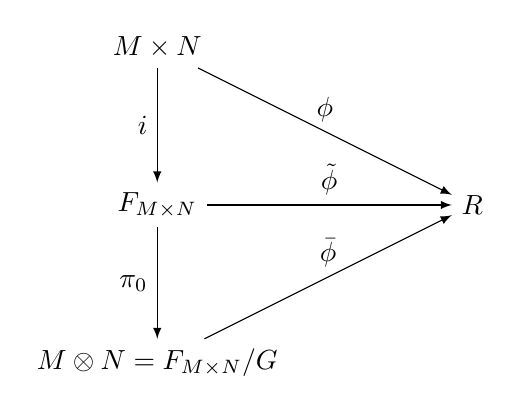
\begin{tikzpicture}
\node (fmn) at (0,0) {$F_{M\times N}$};
\node (R) at  (4,0) {$R$};
\node (mn) at  (0, 2) {$M\times N$};
\node (fmng) at  (0,-2) {$M\otimes N= F_{M\times N}/G$};

\draw[->,>=latex] (mn) to node[above]{$\phi$} (R);
\draw[->,>=latex] (fmn) to node[above]{$\Tilde{\phi}$}(R);
\draw[->,>=latex] (fmng) to node[above]{$\Bar{\phi}$} (R);
\draw[->,>=latex] (mn) to node[left]{$i$}(fmn);
\draw[->,>=latex] (fmn) to node[left]{$\pi_0$} (fmng);

\end{tikzpicture}
\end{center}
\caption{\label{fig:diagcom}Commutatif diagram}
\end{figure}
 
  The following proposition generalizes the theorem and remark to the case of $p$ $K$-modules.  
  
\begin{prop}\label{multitensorprod}
    Let $M_1,\dots,M_p$ be $K$-modules. We define by induction $$M_1 \otimes \dots \otimes M_p = M_1 \otimes (M_2 \otimes \dots \otimes M_p).$$
    Let $f$ be a function from $M_1 \times \dots \times M_p$ into some $K$-module $R$. Then $f$ is $p$-linear if and only if there exists a linear map $\Bar{f}: M_1 \otimes \dots \otimes M_p \to R$ such that $f(x_1,\dots,x_p) = \Bar{f}(x_1 \otimes \dots \otimes x_p)$ for all $(x_i)_i$ in $(M_i)_i$.
\end{prop}

\begin{proof}

We proceed by induction. The initial case, for $p=2$ is already proven. Suppose the result true for $p-1\geq 2$, and let $f$ be a function from $M_1 \times \dots \times M_p$ into $R$. Then if for each $x_p \in M_p$ we call $f_{x_p}$ the function from $M_1 \times \dots \times M_{p-1}$ to $R$ which associates to each $(x_1,\dots,x_{p-1})$ the element $f(x_1,\dots,x_{p-1},x_p)$ of $R$, then we can factor this function through $M_1 \otimes \dots \otimes M_{p-1}$ into $\overline{f_{x_p}}$. And then we can simply define $\overline{f}(x_1 \otimes \dots \otimes x_{p-1} \otimes x_p) = \Bar{f_{x_p}}(x_1 \otimes \dots \otimes x_{p-1})$. 

\end{proof}

\begin{prop} 
    The tensor product of $K$-modules is associative up to isomorphism: we have $$ L\otimes(M \otimes N) \simeq (L\otimes M) \otimes N \;. $$ 
\end{prop}  


\begin{proof}
%% merci beaucoup a Marc Sage. 
%% cette preuve est plus ou moin un copie coller de la preuve sur page 7 de son poly ^_^ <3 
For any $n$ in $N$ we define the mapping
\begin{equation*}
    \begin{split}
        \phi_n : L \times M & \to L \otimes (M \otimes N) \\
        (l,m) & \mapsto l \otimes (m \otimes n).
    \end{split}
\end{equation*}This mapping is bilinear, so we can factor it via 

\begin{equation*}
    \begin{split}
        \overline{\phi}_n : L \otimes M & \to L \otimes (M \otimes N) \\
        l \otimes m & \mapsto l \otimes (m \otimes n).
    \end{split}
\end{equation*}

Since the mapping $n \mapsto \overline{\phi}_n$ is linear, the mapping

\begin{equation*}
    \begin{split}
        \Phi : (L \otimes M) \otimes N & \to L \otimes ( M \otimes N) \\
        (l \otimes m) \otimes n & \mapsto \overline{\phi}_n(l\otimes m )\otimes n = l \otimes (m \otimes n)
    \end{split}
\end{equation*}is linear. 

Similarly, we can fix an $l$ in $L$ and construct 

\begin{equation*}
    \begin{split}
        \psi_l : M \times N & \to (L \otimes M) \otimes N \\
        (m,n) & \mapsto (l \otimes m) \otimes n
    \end{split}
\end{equation*} which we then factor via

\begin{equation*}
    \begin{split}
        \overline{\psi}_l : M \otimes N & \to (L \otimes M) \otimes N \\
        m \otimes n & \mapsto (l \otimes m ) \otimes n.
    \end{split}
\end{equation*}
Once again, the mapping $l \mapsto \overline{\psi}_l$ is linear so this makes the mapping 

\begin{equation*}
    \begin{split}
        \Psi : L \otimes (M \otimes N) & \to (L \otimes M) \otimes N \\
        l \otimes (m \otimes n) & \mapsto \overline{\psi}_l (m \otimes n) = (l \otimes m) \otimes n
    \end{split}
\end{equation*} linear. 

We have that $\Phi$ and $\Psi$ are inverses of each other, so they are bijections, hence the result. 
\end{proof}    

\bigskip
The following proposition gives a commutative property of the tensor product of $K$-modules.

\begin{prop}
    There is a unique isomorphism from $L \otimes M $ to $M \otimes L$ that sends $l \otimes m$ to $m \otimes l$ for each $l$ in $L$ and each $m$ in $M$.
\end{prop}    
    
\begin{proof}
    Let $\phi: L \times M \to M \otimes L$ be the bilinear function that to each $(l,m)$ associates $m \otimes l$ in $M \otimes L$. By the universal property proved in Theorem \ref{prod tens mods}, there is a unique $\Bar{\phi}: L \otimes M \to M \otimes L$ such that $\Bar{\phi}(l \otimes m) = \phi (l,m) = m \otimes l$. Similarly, take $\psi: M \times L \to L \otimes M$ to be the bilinear function that to each $(m,l)$ associates $l \otimes m$. Once again, by the universal property proved in Theorem \ref{prod tens mods}, there is a unique linear map $\Bar{\psi}: M\otimes L \to L \otimes M $ such that $\Bar{\psi}(m \otimes l) = \psi(m,l) = l \otimes m$.
    
    We have $\Bar{\psi}\circ\Bar{\phi} = id_{L\otimes M}$ and $\Bar{\phi}\circ \Bar{\psi} = id_{M \otimes L}$, hence $L \otimes M$ and $M \otimes L$ are isomorphic.
\end{proof}    

%B : il faut virer le diagramme car il y a une partie ou $x_p$ et fixé et puis une ou c'est pas le cas...
   % Commutative diagram \ref{fig:diagcom2} may help illustrate this. 
%\begin{center}
%\begin{tikzpicture}
%\node (N) at  (4,1) {$N$};
%\node (M1timesMp) at (0,4) {$\mathcal{L}(M_1 , \dots , M_p;R)$};
%\node (M1timesMp-1) at  (0, 2) {$\mathcal{L}(M_1, \dots, M_{p-1};R)$};
%\node (M1otimesMp-1) at  (0,0) {$\mathcal{L}(M_1 \otimes \dots \otimes %M_{p-1};R)$};
%\node (M1otimesMp) at (0,-2) {$\mathcal{L}(M_1 \otimes \dots \otimes M_p;R) $};

%\draw[->,>=latex] (M1timesMp) to node[above]{$f$} (R);
%\draw[->,>=latex] (M1timesMp) to node[above]{} (M1timesMp-1);
%\draw[->,>=latex] (M1timesMp-1) to node[above]{$f_{x_p}$} (R);
%\draw[->,>=latex] (M1otimesMp-1) to node[above]{$\overline{f_{x_p}}$} (R);
%\draw[->,>=latex] (M1otimesMp) to node[above]{$\overline{f}$} (R);
%\draw[->,>=latex] (M1timesMp-1) to node [left]{} (M1otimesMp-1);
%\draw[->,>=latex] (M1otimesMp-1) to node[left]{}(M1otimesMp);

%\end{tikzpicture}
%\end{center}
%\caption{\label{fig:diagcom2}Commutatif diagram 2}
%\end{figure}

\begin{remark}
It is possible for the tensor product of two non-trivial $K$-modules to be trivial. For example, if $M \otimes N=\mathbb{Z}/2\mathbb{Z} \otimes \mathbb{Z}/3\mathbb{Z}$ is isopmorphic to $\{0\}$ as for any $m$ and $n$ we have
$m.1_M \otimes n.1_N= mn (3-2)(1_M \otimes 1_N)=mn [(3.1_M \otimes 1_N)-(1_M \otimes 2.1_N)]=
mn[(0.1_M \otimes 1_N)-(1_M \otimes 0.1_N)]=mn[0(1_M \otimes 1_N)-0(1_M \otimes 1_N)=0_{M \otimes N}$.
    
\end{remark}

    \subsection{Properties}
    
    We will now list general properties of the tensor product of $K$-modules. 
  
  \bigskip 
   From the definition of $M \otimes N$ we get immediately the following proposition.
    
    \begin{prop}
     The tensor product $M \otimes N$ is generated by the set of the "\textbf{pure tensors}" $m\otimes n$ for $m$ in $M$ and $n$ in $N$.   
    \end{prop}
    
    \bigskip
    We have shown that $\pi$ is bilinear, so we get the following equalities: 
  \begin{prop}
    For any modules $M$ and $N$, and any elements $m \in M$ and $n \in N$, 
    $$a(m\otimes n)= (am)\otimes n = m \otimes (an)\;,$$
    $$(m+m')\otimes n = m \otimes n + m' \otimes n\;,$$ 
    
    and similarly for the right side. 
      
  \end{prop}  
    
     
    Moreover, Theorem \ref{prod tens mods} has the following important corollary.
    
    \begin{prop}
     For any $K$-module $R$, the module $\mathcal{L}(M,N;R)$ of bilinear maps from $M \times N$ to $R$ is isomorphic to the module $\mathcal{L}(M \otimes N;R)$ of linear maps from $M \otimes N$ to $R$. 
    \end{prop}
   
    
    \begin{proof}
        In the notation of Theorem \ref{prod tens mods}, consider the map $$L : \mathcal{L}(M,N;R) \longrightarrow \mathcal{L}(M\otimes N;R)\;\;,$$ $$\phi \longmapsto \Bar{\phi}\;$$
    clearly well defined on all elements of $\mathcal{L}(M,N;R)$. The map $L$ is linear, as for all $\lambda \in K$ and for all $\phi,\phi_1,\phi_2\in \mathcal{L}(M,N;R)$ 
    \begin{equation*}
        \begin{split}
            & L (\phi_1+\phi_2) = \overline{\phi_1+\phi_2} = \Bar{\phi_1} + \Bar{\phi_2} = L(\phi_1) + L(\phi_2) \\
            & L(\lambda \phi) = \lambda \Bar{\phi} =\lambda L(\phi)
        \end{split}
    \end{equation*} by the universal property of $M \otimes N$. Indeed, $\phi_1 + \phi_2$ can be factored via $\overline{\phi_1 + \phi_2}$ since it is a bilinear map on $M\times N$. As $\phi_1$ can be factored via $\overline{\phi_1}$ and $\phi_2$ can be factored via $\overline{\phi_2}$, $\phi_1 + \phi_2$ can also be factored via $\overline{\phi_1} + \overline{\phi_2}$. But then $\overline{\phi_1 + \phi_2} = \overline{\phi_1} + \overline{\phi_2}$ as the factorisation is unique. 
    
    Similarly, we can factor $\overline{\lambda \phi}$ through $\overline{\lambda \phi}$ and through $\lambda \overline{\phi}$, hence the latter two mappings are the same. 
    


Finally, to show that $L$ is a bijection, take any $f \in \mathcal{L}(M \otimes N;R)$, and consider the function
    %hi Brigitte ^_^
    \begin{equation*}
        \begin{split}
            \phi: M \times N & \to R \\
            (m,n) & \mapsto f (m \otimes n). 
        \end{split}
    \end{equation*}
        This $\phi$ is bilinear, as for all $\lambda \in K$, $m \in M$ and $n \in N$, 
        \begin{equation*}
            \begin{split}
               & \phi(m + m',n) = f((m+m')\otimes n) = f(m\otimes n + m' \otimes n) = f(m\otimes n) + f(m' \otimes n) = \phi(m,n) + \phi(m',n) \\
               & \phi( \lambda m , n) = f( \lambda m \otimes n) = \lambda f(m\otimes n) = \lambda \phi(m,n) ,
            \end{split}
        \end{equation*}
        and similarly on the right hand side. To use the language of Theorem \ref{prod tens mods} we have $\phi = f \circ \pi$. 
        
        This function is also unique, as any other function with the same property would have the same image for all elements of $M \times N$, and as such $L$ is an isomorphism, since every element of $\mathcal{L}(M \otimes N; R)$ has a unique antecedent by $L$. 
        
        The universal property of $M\otimes N$ implies that every bilinear $\phi$ on $M \times N$ can be associated with a unique linear $f$ on $M\otimes N$. Since we have just shown that every linear function on $M \otimes N$ has a unique antecedent, hence the result. 
    
    
    \end{proof}
    
  
  
          
    \begin{remark}
        By the previous proposition, the module $\mathcal{L}(M \otimes N;R)$ is isomorphic to $\mathcal{L}(M,N;R)$. Thus, by proposition \ref{L(M,N;R) iso L(M;L(N;R)}, the modules $\mathcal{L}(M;\mathcal{L}(N;R))$ and $\mathcal{L}(M \otimes N;R)$ are also isomorphic.
    
 
 
   Following Proposition \ref{multitensorprod}, this can be generalized to $p$-linear maps over $p$ modules. 
 \end{remark}

\bigskip



% \vspace{1cm}
 
\section{Links between diverse notions of tensor product and tensors} 

\subsection{A mapping from $M\otimes \dots \otimes M\otimes M^* \otimes \dots \otimes M^*   $ to  $T^p_q(M)$}


%B a B vrai...The following proposition is an immediate corollary of the universal property of the tensor product of modules (see Proposition \ref{multitensorprod}).



\begin{prop} \label{lien tenseurs}
    Suppose $K$ is a commutative ring. Let $M$ be a $K$-module and $p$ and $q$ positive integers. Consider the module $M\otimes \dots \otimes M\otimes M^* \otimes \dots \otimes M^* $, with $p$ occurrences of $M$ and $q$ occurrences of $M^*$.\\
    There exists a unique morphism 
    $$j: M\otimes \dots \otimes M\otimes M^* \otimes \dots \otimes M^*  \to T^p_q(M)$$
    that sends the element $x_1 \otimes\dots \otimes x_p \otimes u_1 \otimes \dots \otimes u_q $ of $ M\otimes \dots \otimes M\otimes M^* \otimes \dots \otimes M^* $\\
    to the element  $x_1 \otimes\dots \otimes x_p \otimes u_1 \otimes \dots \otimes u_q $ of $T^p_q(M)$ 
    (following Remark \ref{pour j}, we recall that this latter expression is the multi-linear form on $(M^*)^p \times M^q$ whose value at $(v_1,  \dots , v_p,y_1,\dots,y_q) $ is the scalar $v_1(x_1) \dots v_p(x_p)u_1(y_1)\dots u_q(y_q)$).
   
   
   
\end{prop}
    
\begin{proof}
Since the map $M^p \times (M^*)^q$ that sends the element $(x_1,  \dots , x_p,u_1,\dots,u_q) $ of $M^p \times (M^*)^q$ to the element $x_1 \otimes\dots \otimes x_p \otimes u_1 \otimes \dots \otimes u_q $ of $T^p_q(M)$ is multi-linear, the proposition is an immediate corollary of the universal property of the tensor product of modules (see Proposition \ref{multitensorprod}). In other words, the morphism $j$ is completely defined by its values on the pure tensors of $M\otimes \dots \otimes M\otimes M^* \otimes \dots \otimes M^*$.

\end{proof}
    
\begin{remark}
    If $M = \mathbb{Z}/{p\mathbb{Z}}$, and $K$ is $\mathbb{Z}$ (so that $M$ is not a free $K$-module), then $T^2_0(M) = \{0\}$ is not isomorph to $M \otimes M$. As such, in this case the morphism $j$ introduced above is not an isomorphism. 
%\textcolor{}{B a A : En effet, d'abord le dual de $M$ comme $\mathbb{Z}$-module est nul, car si $u$ est une forme lineaire sur $M$, pour tout $x$ appartenant a $M$ on a $p.x=0_M$ (on dit que les elements de M sont "de torsion" pour dire ici qu'ils ont un multiple non trivial nul, c'est pour ca que M n'est pas un module libre) et donc  $u(p.x)=u(0_M)=0=pu(x)$, qui montre que $u(x)=0$, donc $u$ est nulle. De $M^*$ nul on deduit $T^2_0(M) = \{0\}$.\\
%Maintenant il faut s'occuper de $M\otimes M$ : tu dis que $1 \otimes 1$ est non nul:\\
%"On the other hand $M\otimes M$ contains $1 \otimes 1$ which is non nul, hence $j$ is not bijective."\\
%mais on n'en sait rien, et du coup il faut suivre Godement:\\}
Indeed, consider the mapping from $M\times M$ to $M$ associating to $(x,y)$ the product $xy$ (that is the multiplication of integers modulo $p$). This is a bilinear non trivial map, and by the universal property of $M\otimes M$, it can be factorized through a linear map on $M\otimes M$, which shows that $M\otimes M$ is not reduced to its zero element. For the case of $T^2(M)$ we have that any element can be uniquely identified by its image of basis element, but $M^* = \{0\}$, and so $T^2(M) = 0$.

%Indeed, an element $g \in T^2_0(M)$ may associate to each elements $u$ and $v$ of $M^*$ the scalar $u(x)v(y)$ for some $x$ and $y$ fixed in $M$. Take any $u,v$ in $M^*$.
   % \begin{equation*}
   % \begin{split}
        %& g(u,v) = u(x)v(y) = u(x + px)v(y + py) \\ 
       %& = xyu(1)v(1) = (p+1)xyu(1)v(1)
    %\end{split}
    %\end{equation*}
    
 %Hence $g(u,v) = 0$ for all $u$ and $v$. But this is true for every element in $T^2_0$, so we must have that $T^2_0 = \{0\}$.
 
  
\end{remark}


\bigskip

\begin{remark}
    We have just shown that while the notions of tensors defined as multi-linear forms and tensors defined as elements of the tensor product of $K$-modules do coincide when the $K$-modules are finitely generated free modules, they are not necessarily identical. We have also seen that the tensor product of two non-trivial $K$-modules can be trivial. 
\end{remark}



\subsection{On tensor product of linear maps}


The results exhibited here above hold not only for the case of tensor products of linear forms, but also for tensor products of linear map with values in $K$-modules. 

\begin{prop}
    Let $L,L',M$ and $M'$ be four $K$-modules. 
    Let $$u : L \to L'$$ and $$v: M \to M' $$ be two linear maps. Then there exists a unique linear map $f$ from $L \otimes M $ to $L' \otimes M'$ such that $f(x \otimes y) = u(x) \otimes v(y)$, for all $x$ in $L$ and $y$ in $M$.
\end{prop}
    
\begin{proof}
    Let $\phi : L \times M \to L' \otimes M'$ be the map that sends $(x,y)$ to $u(x)\otimes v(y)$. We verify that $\phi$ is indeed bilinear: 
    \begin{equation*}
    \begin{split}
       & \phi (\lambda x + \lambda'x',y) = (\lambda x + \lambda' x')\otimes y \\ = 
       & \lambda(x \otimes y) + \lambda' (x'\otimes y) = \lambda\phi(x,y) + \lambda'\phi(x',y)
    \end{split}    
    \end{equation*}
    by bi-linearity of the tensor product, and similarly on the right side. As $\phi$ is bilinear there is a unique linear map $\Bar{\phi}:L\otimes M \to L' \otimes M'$ such that $\Bar{\phi} (x\otimes y) = \phi(x,y)$. We chose $f = \Bar{\phi}$.
\end{proof}
    This unique linear map will now be formally defined. 
\begin{defin}
        Let $L,L',M,M'$ be $K$-modules and $u: L \to L'$ and $v: M \to M'$ be linear maps. The \textbf{tensor product of linear maps} $u$ and $v$ is the unique linear map, noted $u \Tilde{\otimes} v$ that associates to each $l\otimes m$ in $L \otimes M$ the element $u(l) \otimes v(m)$ in $L' \otimes M'$. 
\end{defin}

\paragraph{Notation} The notation $u \Tilde{\otimes} v$ for the tensor product of linear maps $u$ and $v$ is to distinguish $u \Tilde{\otimes} v$ from the element $u \otimes v$ of $\mathcal{L}(L,L') \otimes \mathcal{L}(M,M')$. However, let us remark that the mapping
\begin{equation*}
    \begin{split}
        \mathcal{L}(L;L') \times \mathcal{L}(M;M') & \to \mathcal{L}(L\otimes M; L' \otimes M') \\
        (u,v) & \mapsto u \Tilde{\otimes} v
    \end{split}
\end{equation*}
is bilinear, as this is easily deduced from the fact that, for each pure tensors $x \otimes y \in L \otimes M$, 

\begin{equation*}
    \begin{split}
        & [(\lambda u + \mu u') \Tilde{\otimes} v] (x \otimes y) = (\lambda u + \mu u')(x) \otimes v(y) \\
        & = (\lambda u (x) + \mu u'(x))\otimes v(y) = \lambda u(x)\otimes v(y) + \mu u'(x) \otimes v(y) \\
        & = [\lambda u \Tilde{\otimes} v] (x\otimes y) + [\mu u' \Tilde{\otimes} v ](x \otimes y),
    \end{split}
\end{equation*} and similarly on the right hand side. The universal property of Theorem \ref{prod tens mods} implies that it can be uniquely factored via a linear map
\begin{equation*}
    \begin{split}
        \mathcal{L}(L;L') \otimes \mathcal{L}(M;M') &\to \mathcal{L}(L \otimes M; L' \otimes M') \\
        u\otimes v & \mapsto u \Tilde{\otimes}v
    \end{split}\;\ .
\end{equation*}This morphism is called the \textbf{Kronecker morphism}. In this general case, this morphism is neither injective nor surjective, although it can be shown to be injective in the case of finite dimensional vector spaces. 






\begin{prop}
    Let $L,L',L'',M,M'$ and $M''$ be modules. Let 
    \begin{equation*}
    \begin{matrix}
    u': L \to L' & u'': L' \to L'' \\
    v': M \to M' & v'': M' \to M'' 
    \end{matrix}
    \end{equation*}
    be linear maps. Then
    \begin{equation*}
        (u'' \circ u') \Tilde{\otimes} (v'' \circ v') = (u''\Tilde{\otimes} v'')\circ (u' \Tilde{\otimes} v').
    \end{equation*}
\end{prop}    

\begin{proof}
    Let $x$ be an element of $L$ and $y$ be an element of $M$. 
    We have that
    \begin{equation*}
        \begin{split}
            & [(u'' \circ u')\Tilde{\otimes}(v'' \circ v')](x\otimes y) = (u'' \circ u')(x)\otimes (v'' \circ v')(y) \\
            & = u''(u'(x))\otimes v''(v'(y)) = u''\Tilde{\otimes} v'' (u'(x)\otimes v'(y)) \\
            & = (u''\Tilde{\otimes} v'')\circ(u' \Tilde{\otimes} v') (x\otimes y),
        \end{split}
    \end{equation*}
    for all $x$ in $L$ and $y$ in $M$, hence the result. 
\end{proof}

 
 %In this section the notation $M \otimes N$ refers to a $K$-module made from two existing $K$-modules, and the notation $m\otimes n$ to particular elements of this module. In the previous section, the notation $f\otimes g$ referred to a multilinear form made from two existing multilinear forms. These notations are in fact coherent. An element $f \otimes g$ of the previous section can be seen as an element of $\mathcal{L}(M_1,\dots,M_p;K)\otimes \mathcal{L}(N_1,\dots,N_q;K)$ in this section, assuming of course that $f$ is a multilinear form over $M_1\times \dots \times M_p$ and $g$ is a multi-linear form over $N_1 \times \dots \times N_q$.

%The tensor product of modules is therefore a way of generalizing the tensor product of multilinear forms to all types of modules, because the set of multilinear forms over any Cartesian product of $K$-modules is a $K$-module, as has been previously shown in \ref{multilinearmaps}.This enables us to redefine the tensor product as the operation

\bigskip
We now have different types of tensor products. First, there is the tensor product of linear or multi-linear forms (tensors as commonly used in physics being a particular case of this), as described in \cite{Godement}. Second, we have the tensor product of $K$-modules, and the definition of pure tensors as elements of this tensor product of $K$-modules. Finally, we have just seen the tensor product of linear maps, which we noted $\Tilde{\otimes}$, so as to distinguish $u\otimes v$ from its image by the Kronecker morphism $u \Tilde{\otimes} v$. 




%%%%
\subsection{The special case of tensor product of finitely generated free modules}
 %\textcolor{blue!60! black} {La se serait mieux de passer au produit tensoriel de modules libres de type fini ; du coup pas mal de prop sont a remonter, en simplifiant les preuves souvent immediates grace aux resultats de la section precedente}
In this section $K$ is a commutative ring and $L$ and $M$ are $K$-modules. 

\bigskip

\subsubsection{A base for the tensor product of modules}
We will begin with a technical result which will enable us to determine a base for the tensor product of two finitely generated free modules. 


\begin{prop}\label{direct sum is distributive wrt tensor product}

                for any families of $K$-modules $(L_i)_i$ and $(M_j)_j$,
                \begin{equation*}
                        (\bigoplus_{i} L_i) \otimes (\bigoplus_{j} M_j) \simeq \bigoplus_{i,j} (L_i \otimes M_j).
                \end{equation*}
        \end{prop}

        \begin{proof}
                Consider the function
                \begin{equation*}
                \begin{split}
                        \Pi : (\prod_i L_i) \times (\prod_j M_j) & \to \prod_{i,j} (L_i \otimes M_j) \\
                        ( (l_i)_i ) , (m_j)_j ) & \mapsto (l_i \otimes m_j)_{i,j}.
                \end{split}
                \end{equation*}
                It is bilinear as
                \begin{equation*}
                        \begin{split}
                                \Pi( \lambda(l_i)_i + \mu(l'_i)_i , (m_j)_j) & = ((\lambda l_i + \mu l'_i) \otimes m_j )_{i,j} \\
                                & = (\lambda l_i \otimes m_j + \mu l'_i \otimes m_j)_{i,j} = \lambda (l_i \otimes m_j)_{i,j} + \mu(l'_i \otimes m_j)_{i,j} \\
                                & =\lambda \Pi((l_i)_i,(m_j)_j) + \mu \Pi( (l'_i)_i, (m_j)_j )\;,
                        \end{split}
                \end{equation*}
                and similarly on the right hand side. By the universal property of the tensor product of $K$-modules, there exists therefore a unique linear map,
                determined by the values on the pure tensors
                
\begin{equation*}
                        \begin{split}
                                \overline{\Pi} : (\prod_i L_i) \otimes (\prod_j M_j) & \to \prod_{i,j} (L_i \otimes M_j) \\
                                (l_i)_i \otimes (m_j)_j & \mapsto (l_i \otimes m_j)_{i,j}.
                        \end{split}
                \end{equation*}
                When we compose this linear map with the canonical injection
                \begin{equation*}
                        i : (\bigoplus_i L_i) \otimes (\bigoplus_j M_j)  \to (\prod_i L_i) \otimes (\prod_j M_j)
                \end{equation*}
                we find that the mapping
                \begin{equation*}
                        \begin{split}
                                \Phi : (\bigoplus_i L_i ) \otimes (\bigoplus_j M_j) &\to \bigoplus_{i,j} (L_i \otimes M_j) \\
                                (l_i)_i \otimes (m_j)_j & \mapsto (l_i \otimes m_j)_{i,j}
                        \end{split}
                \end{equation*}
                is linear, as it is a composition of two linear maps, and well defined, as the image of any family with a finite number of non nul elements will be a family with a finite number of non nul elements. 

                For each pair of indices $i,j$ we define
                \begin{equation*}
                        \begin{split}
                        \phi_{i,j} : L_i \times M_j & \to (\bigoplus_i L_i) \otimes (\bigoplus_j M_j) \\
                        (l_i ,m_j) & \mapsto (l_i) \otimes (m_j).
                        \end{split}
                \end{equation*}
                These functions are bilinear, as can be simply verified, so there exists for each $i,j$ a unique linear map
                \begin{equation*}
                        \begin{split}
                                \overline{\phi_{i,j}}: L_i \otimes M_j &\to (\bigoplus_i L_i) \otimes(\bigoplus_j M_j) \\
                                (l_i \otimes m_j) & \mapsto (l_i) \otimes (m_j).
                                \end{split}
                \end{equation*}
                These linear maps can be combined to create a linear map
                \begin{equation*}
                        \begin{split}
                                \Psi : \bigoplus_{i,j} (L_i \otimes M_j) & \to (\bigoplus_i L_i) \otimes (\bigoplus_j M_j) \\
                                (l_i \otimes m_j)_{i,j} & \mapsto (l_i)_i \otimes (m_j)_j 
                        \end{split} 
                \end{equation*}
                which is the inverse of $\Phi$, hence the isomorphism.
        \end{proof}


\bigskip


\begin{prop}
    Let $L$ and $M$ be finitely generated free modules. Let $(a_i)_{1\leq i\leq p}$ be a basis of $L$ and $(b_j)_{1 \leq j \leq q}$ be a basis of $M$. The products $$ (a_i \otimes b_j)_{1\leq i \leq p, 1 \leq j \leq q} $$
    form a basis of $L \otimes M$.\\
    The rank of $L\otimes M$ is the product of the rank of $L$ and the rank of $M$. In particular, if $K$ is a commutative field, then $$ dim(L\otimes M) = dim(L)dim(M). $$
\end{prop}    
    
\begin{proof}
%    We start by choosing any element $m$ in $M$. For all $l$ in $L$, we have that there exists $\lambda_1, \dots, \lambda_p$ such that  $l = \sum_i \lambda_i a_i %$. Because $M$ is also finitely generated, with basis $(b_j)_j$, there exists $\mu_1, \dots, \mu_q$ such that $m = \sum_j (\mu_j  b_j)$. Using the bi-linearity of %the tensor product, we find \begin{equation*}
 %       \begin{split}
 %           l \otimes m & = \sum_i \lambda_i (a_i \otimes m ) \\
 %           & = \sum_i \sum_j \lambda_i \mu_j (a_i \otimes b_j).
 %       \end{split}
 %   \end{equation*}   .
 %   As such, any element of $L \otimes M $
%can be written as a linear combination of elements of $(a_i \otimes b_j)_{i,j}$, and so the $(a_i \otimes b_j)_{i,j}$ generate $L \otimes M$.    
    By Proposition \ref{direct sum is distributive wrt tensor product} we have 
    \begin{equation*}
        \begin{split}
            L \otimes M = (\bigoplus_i K a_i)_i \otimes (\bigoplus_j K b_j)_j \simeq \bigoplus_{i,j} K (a_i \otimes b_j).
        \end{split}
    \end{equation*}
\end{proof}
% merci Brigitte ^_^

\vspace{1,5cm}
\subsubsection{Isomorphism between $M\otimes \dots \otimes M\otimes M^* \otimes \dots \otimes M^*$ and  $T^p_q(M)$}
\bigskip
We come back to the mapping $j$ from $M\otimes \dots \otimes M\otimes M^* \otimes \dots \otimes M^* $ to  $T^p_q(M)$ of Proposition \ref{lien tenseurs}.

\begin{prop}
    Suppose  $M$ be a free $K$-module of finite type, $p$ and $q$ positive integers and consider the module $M\otimes \dots \otimes M\otimes M^* \otimes \dots \otimes M^* $, with $p$ occurrences of $M$ and $q$ occurrences of $M^*$.\\
    The map 
    $$j: M\otimes \dots \otimes M\otimes M^* \otimes \dots \otimes M^*  \to T^p_q(M)$$
    that sends the element $x_1 \otimes\dots \otimes x_p \otimes u_1 \otimes \dots \otimes u_q $ of $ M\otimes \dots \otimes M\otimes M^* \otimes \dots \otimes M^* $\\
    to the element  $x_1 \otimes\dots \otimes x_p \otimes u_1 \otimes \dots \otimes u_q $ of $T^p_q(M)$ 
    is an isomorphism.
\end{prop}

\begin{proof}
    

 Suppose that $M$ is finitely generated, with basis $(a_i)_{1 \leq i \leq n}$. Then we have that the elements
    \begin{equation*}
        (a_{i_1} \otimes \dots \otimes a_{i_p} \otimes a^{j_1} \otimes \dots \otimes a^{j_q})_{1 \leq i_1 , \dots, i_p , j_1  \dots, j_p \leq n } 
    \end{equation*} form a basis of $M\otimes \dots \otimes M \otimes M^* \otimes \dots \otimes M^*$, and their images by $j$ form a basis of $T^p_q(M)$: $j$ is an isomorphism.
   
\end{proof}

\vspace{1,5cm}
\subsubsection{Tensor product of linear maps and Kronecker product of matrices}
\bigskip
    Let $L$, $L'$, $M$ and $M'$ be free $K$-modules of finite type. Let $$ u : L \to L'  \; \textrm{and} \; v: M \to M' $$ be linear maps. We are going to show how to write the matrix of $u \Tilde{\otimes} v$ as a function of the matrices of $u$ and $v$.

  
\bigskip
    Let us consider $\mathcal{A}=(a_i)_{1 \leq i \leq p}$, $\mathcal{B}=(b_j)_{1 \leq j \leq q}$, $\mathcal{C}=(c_k)_{1 \leq k \leq r}$ and $\mathcal{D}=(d_l)_{1 \leq l \leq s}$ bases of $L$, $L'$, $M$ and $M'$ respectively. Let $A = (\alpha_{ij})_{(i,j) \in \{1,\dots,p\}\times \{1,\dots,q\}}$ and $B = (\beta_{kl})_{(k,l) \in \{1,\dots,r\}\times\{1,\dots,s\}}$ be the matrices of $u$ and $v$ in these bases: 
    \begin{equation*}
        A=\mathcal{M}_{\mathcal{A}, \mathcal{B}}(u) = \begin{bmatrix}
        \alpha_{11} & \dots &   \alpha_{1p} \\
        \vdots & \ddots & \vdots \\
        \alpha_{q1} & \dots & \alpha_{qp}
        \end{bmatrix}\;,
    \end{equation*}
    
    \begin{equation*}
        B=\mathcal{M}_{\mathcal{C}, \mathcal{D}}(v) = \begin{bmatrix}
        \beta_{11} & \dots &   \beta_{1r} \\
        \vdots & \ddots & \vdots \\
        \beta_{s1} & \dots & \beta_{sr}
        \end{bmatrix}\;.
    \end{equation*}
    For the sake of convenience, we identify in the following elements of the module $L$, $L'$, $M$ and $M'$ with their column matrices of coordinates in the chosen bases. If $x$ and $y$ are elements of $L$ and $M$, then $(u\Tilde{\otimes} v) (x,y)$ will be the element $x'\otimes y'$ with 
    \begin{equation*}
        x' = 
        \begin{pmatrix}
        x'_1 = \sum_i \alpha_{1i}x_i\\
        \vdots \\
        x'_q = \sum_i \alpha_{qi}x_i
        \end{pmatrix}
    \end{equation*}
    
    and 
    \begin{equation*}
        y' = 
        \begin{pmatrix}
        y'_1 = \sum_i \beta_{1i}y_i \\
        \vdots \\
        y'_s = \sum_i \beta_{si}y_i
        \end{pmatrix}\;.
    \end{equation*} 
    
  
  %  Nous choisissons de faire croitre les indices des $c_k$ avant ceux des $a_i$ et ceux des $d_l$ avant ceux des $b_j$.}
    In order to write the tensor products $x \otimes y$ and $x' \otimes y$ as column matrices, we will need to chose a way of ordering the elements of the bases $(a_i \otimes c_k)_{1\leq i \leq p, 1\leq k \leq r}$ or $L \otimes M$ and $ (b_j \otimes d_l)_{1 \leq j \leq q, 1 \leq l \leq s} $ of $L'\otimes M'$.
    We will chose to increase the indices of the $c_k$ before the $a_i$ and the $d_l$ before the $b_j$.
    
    
    Then, we can write the tensor product of vectors in the form 
    \begin{equation*}
        x \otimes y = 
        \begin{pmatrix}
        x_1 y_1 \\
        \vdots \\
        x_1 y_r \\
        x_2 y_1 \\
        \vdots \\
        x_2 y_r \\
        \vdots \\
        x_p y_1 \\
        \vdots \\
        x_p y_r 
        \end{pmatrix}\;\;\text{and}\;\;
        x' \otimes y' = \begin{pmatrix}
        x'_1 y'_1 \\
        \vdots \\
        x'_1 y'_r \\
        x'_2 y'_1 \\
        \vdots \\
        x'_2 y'_s \\
        \vdots \\
        x'_q y'_1 \\
        \vdots \\
        x'_q y'_s
        \end{pmatrix}.
    \end{equation*}
    
    We note that this convention of having the $y_k$ change before the $x_i$ and the $y'_l$ change before the $x'_j$  is completely arbitrary. It is possible to use a different symbolic formalism, for instance alternating the $x_i$ before the $y_i$, and arrive at the result so long the same formalism is used during the entirety of the calculation. 
    
   When the bases are ordered according to the previous convention, the matrix of $u\Tilde{\otimes} v$ is equal to 
    \begin{equation*} 
    \begin{bmatrix}
    \alpha_{11} \beta_{11} & \dots & \alpha_{11} \beta_{1r} & \alpha_{12} \beta_{11} & \dots & \alpha_{12} \beta_{1r} & \dots & \alpha_{1p} \beta_{11} & \dots & \alpha_{1p} \beta_{1r} \\
    
    \alpha_{11} \beta_{21} & \dots & \alpha_{11} \beta_{2r} & \alpha_{12} \beta_{21} & \dots & \alpha_{21} \beta_{r2} & \dots & \alpha_{p1}\beta_{21} & \dots & \alpha_{p1}\beta_{2r} \\
    \vdots & & & & & & & & \vdots \\
    \alpha_{11} \beta_{s1} & \dots & \alpha_{11} \beta_{sr} & \alpha_{12} \beta_{s1} & \dots & \alpha_{12} \beta_{sr} & \dots & \alpha_{1p}\beta_{s1} & \dots & \alpha_{1p}\beta_{sr} \\
    
    
    \alpha_{21} \beta_{11} & \dots & \alpha_{21} \beta_{1r} & \alpha_{22} \beta_{11} & \dots & \alpha_{22} \beta_{1r} & \dots & \alpha_{2p} \beta_{11} & \dots & \alpha_{2p} \beta_{1r} \\
      \vdots & & & & & & & & \vdots \\
    \alpha_{21} \beta_{s1} & \dots & \alpha_{21} \beta_{sr} & \alpha_{22} \beta_{s1} & \dots & \alpha_{22} \beta_{sr} & \dots & \alpha_{2p}\beta_{s1} & \dots & \alpha_{2p}\beta_{sr} \\
    
    
    \vdots & & & & & & & & \vdots \\
    \vdots & & & & & & & & \vdots \\
    
    \alpha_{q1} \beta_{11} & \dots & \alpha_{q1} \beta_{1r} & \alpha_{q2} \beta_{11} & \dots & \alpha_{q2} \beta_{r1} & \dots & \alpha_{qp} \beta_{11} & \dots & \alpha_{qp} \beta_{1r} \\
    
    \vdots & & & & & & & & \vdots \\
    
    \alpha_{q1} \beta_{s1} & \dots & \alpha_{q1} \beta_{sr} & \alpha_{q2} \beta_{s1} & \dots & \alpha_{q2} \beta_{sr} & \dots & \alpha_{qp} \beta_{s1} & \dots & \alpha_{qp} \beta_{sr} \\
    
    
    \end{bmatrix}\;.
    \end{equation*}
    
    We can see that this matrix is obtained from the matrix $A$ of $u$ replacing each coordinate $\alpha_{ij}$ by the matrix block $\alpha_{ij}B$.
    
    This is sometimes called the \textbf{Kronecker Product} of two matrices and noted $A \otimes B$.
    
.
  
  \begin{remark}
  Were we to adopt the convention of having the $x_i$ change before the the $y_k$ and the $x'_j$ change before the $y'_l$, the matrix of $A \otimes B$ would be the matrix composed of the blocks $b_{ij}A$, rather than the blocks $a_{}ijB$ as is with the current convention. 
  \end{remark}
  
  


%%%%%%%%
%%%%%%%%
%%%%%%%%
%%%%%%%%
%%%%%%%%
%%%%%%%%
%%%%%%%%
%%%%%%%%
%%%%%%%%
%%%%%%%%
%%%%%%%%
%%%%%%%%
%%%%%%%%
%%%%%%%%
%%%%%%%%
%%%%%%%%
%%%%%%%%
%%%%%%%%
%%%%%%%%
%%%%%%%%
%%%%%%%%
%%%%%%%%
%%%%%%%%
%%%%%%%%
%%%%%%%%
%%%%%%%%
%%%%%%%%

\chapter{Hypermatrices and tensors}
In this section, $F$ will denote a commutative field.


Hypermatrices are generalizations of matrices to families of scalars with more than two indexes. We will also see that they can be seen as representing the coefficients in a given basis, or set of bases, of a tensor. 


\paragraph{Notation} We will sometimes use the notation $\langle n \rangle$ to denote the set $\{1,\dots,n\}$.


\section{Basic definitions}
\begin{defin}
        A function  $f: \langle n_1 \rangle \times \dots \times \langle n_d \rangle \to F$ will be referred to as a \textbf{hypermatrix} of order $d$.

\end{defin}

\paragraph{Notation}
 The set of hypermatrices on $n_1, \dots n_d$ with coefficients in the field $F$ will be denoted $F^{n_1 \times \dots \times n_d}$.

A hypermatrix can also be represented in the form $A = [a_{i_1 \dots i_d}]$ with $i_k \in \langle n_k \rangle$ for $k \in \langle d \rangle$.
 A hypermatrix of order $2$ is a standard matrix, and as such the set of $m \times n$ matrices over $F$ can be referred to as either $\mathcal{M}_{m \times n}(F)$ or $ F ^{m \times n}$.

Much as with matrices, we define termwise addition in the following manner: if $A = [a_{i_1 \dots i_d}]_{i_1 \in \langle n_1 \rangle, \dots, i_d \in \langle n_d \rangle}$ and $B = [b_{i_1 \dots i_d}]_{i_1 \in \langle n_1 \rangle ,\dots, i_d \langle n_d \rangle}$ are two hypermatrices, of $F^{n_1 \times \dots \times n_d}$, then
\begin{equation*}
        A + B = [a_{i_1 \dots i_d} + b_{i_1 \dots i_d} ]_{i_1 \in \langle n_1 \rangle ,\dots, i_d \in \langle n_d \rangle}
\end{equation*}
will be their sum. For scalar multiplication, if $\lambda$ is a scalar of $F$, and $A = [a_{i_1 \dots i_d}]_{i_1 \in \langle n_1 \rangle ,\dots, i_d \in \langle n_d \rangle}$ is a hypermatrix, then
\begin{equation*}
        \lambda A = [\lambda a_{i_1 \dots i_d}]_{i_1 \in \langle n_1 \rangle ,\dots, i_d \in \langle n_d \rangle}
\end{equation*}
will be the their product.

We define the standard basis of $F^{n_1 \times \dots \times n_d}$ to be $\mathcal{E} = \{ E_{i_1 \dots i_d}: i_1 \in \langle n_1 \rangle , \dots , i_d \in \langle n_d \rangle \} $ where $ E_{i_1 \dots i_d}$ denotes the hypermatrix with a $(i_1, \dots, i_d)$ coordinate of $1$ and zeros everywhere else.

The standard matrix multiplication can be generalized to hypermatrices.

\begin{defin}
        Let $X_1 = (x_{ij}^1) \in F^{m_1 \times n_1}, \dots , X_d = (x_{ij}^d) \in F^{m_d \times n_d}$ are matrices and $A = [a_{i_1 \dots i_d}] \in F^{n_1 \times \dots \times n_d}$ is a hyper matrix, their mutli-linear matrix product is
        \begin{equation*}
                A' = (X_1, \dots, X_d) \cdot A = [a'_{i_1 \dots i_d}] \in F^{m_1 \times \dots \times m_d} 
        \end{equation*}
        defined by
        \begin{equation*}
                a'_{i_1 \dots i_d} = \sum_{k_1, \dots, k_d} x^1_{i_1 k_1}\dots x^d_{i_d k_d}a_{k_1 \dots k_d}.
        \end{equation*}
\end{defin}

We have the following properties:

\begin{prop}
    If $A \in F^{n_1 \times \dots \times n_d}$ is a hypermatrix, and for $i \in \langle d \rangle$ let $X_i \in F^{l_i \times m_i}$ and $Y_i \in F^{m_i \times n_i}$ are matrices, then 
    \begin{equation*}
        (X_1,\dots,X_d)\cdot ((Y_1,\dots,Y_d)\cdot A) = (X_1 Y_1, \dots, X_d Y_d)\cdot A. 
    \end{equation*}
\end{prop}

\begin{proof}
    By calculating we have 
    \begin{equation*}
        \begin{split}
            & (X_1,\dots,X_d)\cdot ((Y_1,\dots,Y_d)\cdot A)  \\
            &  = (X_1,\dots,X_d) \cdot \left[ \sum_{k_1,\dots,k_d}^{n_1, \dots, n_d} y^1_{j_1 k_1} \dots y^d_{j_d k_d} \cdot a_{k_1 \dots k_d} \right]_{j_1\in \langle m_1 \rangle, \dots , j_d \in \langle m_d \rangle} \\
            & = \left[ \sum_{j_1, \dots, j_d}^{n_1, \dots n_d} x^1_{i_1 j_1} \dots x^d_{i_d j_d} \sum_{k_1 , \dots, k_d}^{n_1 ,\dots, n_d} y^1_{j_1 k_1} \dots y^d_{j_d k_d} \cdot a_{k_1 \dots k_d} \right]_{i_1 \in \langle l_1 \rangle, \dots , i_d \in \langle l_d \rangle} \\
            & = \left[ \sum_{j_1 , \dots, j_d } \sum_{k_1 , \dots, k_d} x^1_{i_1 j_1}y^1_{j_1 k_1} \dots x^d_{i_d j_d}y^d_{j_d k_d} a_{k_1 \dots k_d} \right]_{i_1 \in \langle l_1 \rangle, \dots , i_d \in \langle l_d \rangle} \\
            & = \left[ \sum_{k_1 , \dots, k_d} (\sum_{j_1} x^1_{i_1 j_1}y^1_{j_1 k_1}) \dots (\sum_{j_d} x^d_{i_d j_d}y^d_{j_d k_d}) a_{k_1 \dots k_d} \right]_{i_1 \in \langle l_1 \rangle, \dots , i_d \in \langle l_d \rangle} \\
            & = (X_1 Y_1,\dots ,X_d Y_d) \cdot A.
        \end{split}
    \end{equation*}
\end{proof}

\begin{prop}
    If $A$ and $B$ are hypermatrices in $F^{n_1 \times \dots \times n_d}$, $\alpha$ and $\beta$ are scalars and for $k \in \langle d \rangle$ $X_k \in F^{m_k \times n_k}$ are matrices, then 
   $$ (X_1 , \dots , X_d) \cdot (\alpha A + \beta B) = \alpha ((X_1, \dots, X_d) \cdot A) + \beta((X_1, \dots, X_d)\cdot B).$$ 
\end{prop}

\begin{proof}
    Once again by calculating we find
    \begin{equation*}
        \begin{split}
            & (X_1, \dots , X_d) \cdot [\alpha a_{i_1 \dots i_d} + \beta b_{i_1 \dots i_d}]_{i_1 \in \langle n_1 \rangle, \dots , i_d \in \langle n_d \rangle} = \\
            & \left[ \sum_{k_1 , \dots , k_d} x^1_{i_1 k_1} \dots x^d_{i_d k_d} (\alpha a_{i_1 \dots i_d} + \beta b_{i_1 \dots i_d}\right]_{i_1 \in \langle n_1 \rangle, \dots , i_d \in \langle n_d \rangle} \\
            & = \alpha \left[ \sum_{k_1 , \dots ,k_d} x^1_{i_1 k_1} \dots x^d_{i_d k_d} a_{k_1 \dots k_d} \right]_{i_1 \in \langle n_1 \rangle, \dots , i_d \in \langle n_d \rangle} + \beta \left[ \sum_{k_1, \dots , k_d}x^1_{i_1 k_1} \dots x^d_{i_d k_d} b_{k_1 \dots k_d} \right]_{i_1 \in \langle n_1 \rangle, \dots , i_d \in \langle n_d \rangle} \\
            & = \alpha (X_1, \dots, X_d) \cdot A + \beta (X_1, \dots, X_d) \cdot B. 
        \end{split}
    \end{equation*}
\end{proof}


\begin{defin}
        If $\pi \in \mathfrak{S}_d$ is a permutation, and $A = [a_{i_1 \dots i_d}]_{i_1 \in\langle n_1 \rangle,\dots,i_d \in\langle nd \rangle}$ is a hypermatrix of order $d$, then we define the \textbf{$\pi$-transpose of $A$} to be
        \begin{equation*}
                A^\pi = [a_{\pi(i_1)\dots\pi(i_d)}]_{i_1 \in \langle n_1 \rangle,\dots,i_d \in \langle n_d \rangle}.
        \end{equation*}

\end{defin}



The space of $F^{n_1 \times n_p}$ of order $d$ hypermatrices on a field $F$ is a vector space for these operations. Indeed, it is an abelian group with a scalar multiplication that is distributive with regards to the addition operation.


\paragraph{Hypermatrices and tensors}
Let $V_1, \dots, V_d$ are finitely generated free vector spaces of dimension $n_1, \dots, n_d$ over the field $F = \mathbb{R}$ or $F = \mathbb{C}$, with respective bases $\mathcal{B}^1, \dots, \mathcal{B}^d$, where each $\mathcal{B}^i = \{b_1^i, \dots, b_{n_i}^i\}$.
If the tensor $T \in V_1 \otimes \dots \otimes V_d$ has the structure constants or coordinates in the basis $(b^1_{i_1} \otimes \dots \otimes b^d_{i_d})_{i_1 \in \langle n_1 \rangle, \dots , i_d \in \rangle n_d \rangle}$ of $(a_{i_1 \dots i_d})_{i_1 , \dots , i_d}$ then we can represent it in the basis as the hypermatrix
\begin{equation*}
    A = [a_{i_1 \dots i_d}]\in F^{n_1 \times \dots \times n_d}.
\end{equation*}

Furthermore, if $\mathcal{B}'^1, \dots, \mathcal{B}'^d$ is a second set of bases for $V_1, \dots, V_d$, and $X_1, \dots, X_d$ are the respective change of basis matrices from $\mathcal{B}^1, \dots , \mathcal{B}^d$ to $\mathcal{B}'^1 , \dots, \mathcal{B}'^d$, then hypermatrix of $T$ in the new set of bases is 
\begin{equation*}
    A' = (X_1, \dots, X_d) \cdot A.
\end{equation*}

\begin{defin}
        Let $F$ be a field and let  $u^1 \in F^{n_1}, u^2 \in F^{n_2}, \dots, u^d \in F^{n_d} $ be vectors.
        Their \textbf{Segre outer product}, noted $ \otimes b \otimes c$ is defined as
        \begin{equation*}
                \begin{split}
                        [u^1_{i_1} u^2_{i_2} \dots u^d_{i_d}]_{i_1 = 1 i_2 = 1 \dots i_d =1}^{n_1 n_2 \dots n_d}
        .        \end{split}
        \end{equation*}
\end{defin}

The Segre outer product can help us to define an isomorphism between $F^{n_1} \otimes \dots \otimes F^{n_d}$ and $F^{n_1 \times \dots \times n_d}$ when $F$ is $\mathbb{R}$ or $\mathbb{C}$ (and possibly some other fields, but it is best to avoid overgeneralizing and thereby including pathological cases). Indeed, consider the Segre map
\begin{equation*}
    \begin{split}
    \phi : F^{n_1} \times \dots \times F^{n_d} & \to F^{n_1 \times \dots \times n_d} \\
    (u^1, \dots, u^d) & \mapsto u^1 \otimes \dots \otimes u^d.
    \end{split}
\end{equation*}
 It is bilinear, and as such by the universal property of the tensor product of $F$-modules there is a unique $\theta : F^{n_1} \otimes \dots \otimes F^{n_d}$ such that $\theta (u^1 \otimes \dots \otimes u^d ) = u^1 \otimes \dots \otimes u^d$. This mapping is evidently injective, and since $F^{n_1 \times \dots \times n_d}$ and $F^{n_1}\otimes \dots \otimes F^{n_d}$ have the same dimension, it is an isomorphism. 
As such, we have just proved the following result
\begin{prop}
    Let $F$ be a the field $\mathbb{R}$ or $\mathbb{C}$ and $n_1, \dots, n_d$ be positive integers. The vector spaces $F^{n_1 \times \dots \times n_d}$ and $F^{n_1} \otimes \dots \otimes F^{n_d}$ are isomorphic. 
\end{prop}

\begin{defin}
        Let $A = [a_{i_1 \dots i_p}] \in F^{n_1 \times \dots \times n_p} $ and $B = [b_{j_1 \dots j_q}] \in F^{m_1 \times \dots \times m_q} $ be hypermatrices.
        Their \textbf{outer product of hypermatrices} noted $A \otimes B$ is the hypermatrix
        \begin{equation*}
                A \otimes B = [a_{i_1 \dots i_p}b_{j_1 \dots j_q}] \in F^{n_1 \times \dots \times n_p \times m_1 \times \dots \times m_q}.
        \end{equation*}
\end{defin}

\subsection{Some useful concepts}

The terminology \textit{mode}, when used to refer to a hypermatrix, will designate one of its dimensions. For example, if $A \in F^{2 \times 3 \times 4}$ is  a hypermatrix, its first mode, or mode $1$ will be two, second mode $3$, and third mode $4$.

\begin{defin}
        Let $A = [a_{i_1 \dots i_d}]_{i_1 \in \langle n_1 \rangle , \dots, i_d \in \langle n_d \rangle}$ be a hypermatrix. The \textbf{mode $q$ fibers} of $A$ are the vectors formed by fixing all the indices but the $q$ mode index.
\end{defin}

The mode $q$ fibers are noted $a_{i_1 \dots i_{q-1}:i_{q +1}\dots i_d}$.

To illustrate this, if $A$ is as before an element of $F^{n_1 \times \dots \times n_d}$, then the mode $q$ fibers of $A$ will be vectors of the form

\begin{equation*}
        \begin{split}
            a_{i_1\dots i_{q-1}:i_{q+1}\dots i_d} = 
            \begin{pmatrix}
            a_{i_1\dots i_{q-1}1 i_{q+1}\dots i_d} \\
            \vdots \\
            a_{i_1\dots i_{q-1}n_q i_{q+1}\dots i_d} \\
            \end{pmatrix}
        \end{split}
\end{equation*}

Fibers are the hypermatrix analogue of rows and columns of a matrix. In fact, the rows of a matrix are its mode $1$ fiber, and its columns are its mode $2$ fibers.

\begin{defin}
Given a hypermatrix of order $d$ $\mathcal{X} \in F^{n_1 \times \dots \times n_d}$, the \textbf{mode $k$ flattening} of $\mathcal{X}$ is the matrix noted $X^{(k)}$ whose columns are the mode $i$ fibers of $\mathcal{X}$, arranged in reverse lexicographical order.
\end{defin}

Reverse lexicographical order simply means that the leftmost index will vary first, then the second leftmost, and so on, with the rightmost index will vary last. It is the lexicographical order applied to the reverse of each string of indices. For example, given a hypermatrix of order $4$ where $n_1 = n_2 = n_3 =n_4 = 2$, if we chose to take its mode $2$ representation, we will have a $2 \times 8$ matrix with columns 
\begin{equation*}
        X^{(2)} = \begin{bmatrix} x_{1:11} & x_{2:11} & x_{1:21} & x_{2:21} & x_{1:12} & x_{2:12} & x_{1:22} & x_{2:22} \end{bmatrix}.
\end{equation*}

More generally, the mode $k$ flattening is described by mapping each $x_{i_1 \dots i_k \dots i_d}$ in the hypermatrix to $x_{i_k j}$ in the mode $k$ flattening, where
\begin{equation*}
        j = 1 + \sum_{l = 1,l \neq k}^d (i_l -1)(\prod_{ m = 1,m \neq k}^{l-1} n_m).
\end{equation*}


%%%%%%%%
%%%%%%%%
%%%%%%%%
%%%%%%%%
%%%%%%%%
%%%%%%%%
%%%%%%%%
%%%%%%%%
%%%%%%%%

%%%%%%%%
%%%%%%%%
%%%%%%%%
%%%%%%%%
%%%%%%%%
%%%%%%%%
%%%%%%%%
%%%%%%%%
\subsection{Alternative matrix products}
In addition to the Kronecker product, there are other possible matrix products. We will describe two of them, the Khatri-Rao product and the Hadamard product, although other types, such as the Semi-Tensor product and the Tracy-Singh product, also exist. Furthermore, we note that the formalism we have used to describe the Khatri-Rao product is not unique, and that other ways of defining this product exist.

\begin{defin}
        Let $A \in F^{l \times n}$ and $B \in F^{m \times n}$ be two matrices with the same number of columns. The \textbf{Khatri-Rao product} of $A$ and $B$, noted $A \odot B$, is the $lm \times n$ matrix whoses columns are the Kronecker products of the corresponding columns of $A$ and $B$.
\end{defin}

To illustrate this, suppose
\begin{equation*}
        A = \begin{bmatrix}
                a_{11} & \dots & a_{1n} \\
                \vdots & \ddots & \vdots \\
                a_{l1} & \dots & a_{ln} 
        \end{bmatrix}
\end{equation*}

and

\begin{equation*}
        B = \begin{bmatrix}
                b_{11} & \dots & b_{1n} \\
                \vdots & \ddots & \vdots \\
                b_{m1} & \dots & b_{mn}
        \end{bmatrix}.
\end{equation*}

Then $A \odot B$ will take the form

\begin{equation*}
        A \odot B = \begin{bmatrix}
                a_{11} b_{11} & \dots & a_{1n}b_{1n} \\
                \vdots & \ddots & \vdots \\
                a_{11} b_{m1} & \dots & a_{1n}b_{mn} \\
                \vdots & \ddots & \vdots \\
                \vdots & \ddots & \vdots \\
                a_{l1} b_{11} & \dots & a_{ln} b_{1n} \\
                \vdots & \ddots & \vdots \\
                a_{l1} b_{m1} & \dots & a_{ln} b_{mn}
                \end{bmatrix}
\end{equation*}
using the previous formalism of varying the indices of the second matrix before those of the first.


\begin{defin}
        Let $A \in F^{m \times n}$ and $B \in F^{m \times n}$ be two matrices with the same dimensions. Their \textbf{Hadamard product}, noted $A \ast B$ is the $m \times n$ matrix whose elements are the products of the corresponding elements of $A$ and $B$.
\end{defin}

To illustrate this, suppose

\begin{equation*}
        A = \begin{bmatrix}
                a_{11} & \dots & a_{1n} \\
                \vdots & \ddots & \vdots \\
                a_{m1} & \dots & a_{mn} 
        \end{bmatrix}
\end{equation*}

and


\begin{equation*}
        B = \begin{bmatrix}
                b_{11} & \dots & b_{1n} \\
                \vdots & \ddots & \vdots \\
                b_{m1} & \dots & b_{mn}
        \end{bmatrix}.
\end{equation*}

The Hadamard product will be

\begin{equation*}
        A \ast B = \begin{bmatrix}
                a_{11}b_{11} & \dots & a_{1n}b_{1n} \\
                \vdots & \ddots & \vdots \\
                a_{m1}b_{m1} & \dots & a_{mn}b_{mn}
        \end{bmatrix}.
\end{equation*}

\section{Graphs, hypergraphs, and networks}

This section will introduce the basic terminology used to describe graphs, networks and hypergraphs.

\begin{defin}
        A \textbf{graph} $G = (V_G,E_G)$ is a set of nodes (or vertices) $V_G$ and a set of edges between those nodes $E_G\subseteq V_G \times V_G$.
\end{defin}

Graphs are also sometimes referred to as \textbf{networks} and we will use both terminologies.
For the sake of simplicity, we will assume that for a finite graph, the nodes are labeled $1,\dots,n$ where $n$ is the number of nodes. We will also consider exclusively finite graphs.

A graph is called \textbf{simple} if it has no loops and at most one edge between each pair of nodes. A \textbf{multigraph} is a graph with multiple edges between nodes. 

The concept of a graph can be generalized to a hypergraph, by weakening the condition that edges must be pairs.
\begin{defin}
        A \textbf{hypergraph} $H = (V_H,E_H)$ is a collection of vertices or nodes along with a set of hyperedges $E_H \subseteq \mathcal{P}(V_H)$ linking those nodes.

\end{defin}
In both hypergraphs and graphs, edges can be undirected or directed, and weighted or unweighted.

\begin{defin}
        A \textbf{directed graph} or \textbf{digraph} is one where the edges $(a,b)$ and $(b,a)$ are distinct. In other words, edges in a directed graph have a direction from one node to another.
\end{defin}



%%%%%%%%%%
\subsection{Multiplex networks}

Graphs and networks are frequently used to represent data and their interactions. Beyond the visualization of the interaction network (often impossible due to the size of the network), this representation is useful for data analysis and to infer, from a topological analysis of the graph, underlying properties in the data set.
In molecular biology, new technologies provide a huge quantity of heterogeneous data, that can be interpreted as interactions of the biological components at different scales: protein-protein interactions, gene regulation through transcription factors, gene regulation through non-codant RNA, signalling pathways, correlation of expression levels... \cite{lenovere}. While it is important to consider these data as a whole, there is also evidence that it is better to study each of these networks separately, rather than lumping them together into a single network \cite{didier}.  
Multiplex networks are composed of several layers of simple (monoplex) networks. Each layer shares the same set of nodes, but their edges belong to different categories (they have a different meaning).
%For instance, in biology, \textbf{multiplex networks} designate a certain type of multigraph \textcolor{}{No: we distinguish the layers; not to be confused with aggregated graph}. The edges designate interactions between different biological components (typically genes) at different levels. For example, one layer may represent interactions between proteins associated with genes, whilst another may represent interactions between messenger RNA associated with the same genes. 
%Another way of viewing a multiplex can be as a family of graphs whose node sets are all identical, or as a single node set with multiple edge sets. 
Hence, multiplex allow to encode all the different type of interactions between the components, while keeping them separate. An illustration of this is given Figure \ref{multiplex}.% In other words, a multiplex network is a set of nodes $N$ with multiple edge sets $E_1, \dots, E_d$. 

\begin{figure}
\centerline{
    \includegraphics[scale = .5]{multiplex_white.png}}
    \caption{A multiplex network}
    \label{multiplex}
\end{figure}

We need efficient methods to mine and analyse multiplex networks despite their huge size. For example, in \cite{valdeolivas} is proposed a random walk with restart method to predict key components around a gene of interest.
Tensors can be used to encode multiplexes (cf the following subsections), and then could shed new light on the data and their structure.


%%%%%%%%%
\subsection{Some uses of hypermatrices}

Hypermatrices can be used to encode hypergraphs and multiplexes.
For hypergraphs, if the hypergraph contains $n$ nodes, it can be coded as an order $n$ hypercubical hypermatrix will all indices in $\langle n + 1 \rangle$.
To the hypergraph $H = (V,E)$ we can associate the hypermatrix $A_H = [a_{i_1 \dots i_{n}} \in \mathbb{R}^{n+1 \times \dots \times n+1}$ such that each $a_{i_1 \dots i_n}$ is the weight of the hyperedge between nodes $i_1, \dots,i_n$. Of course, this will only work for hyperedges of size $n$, which is why we add a "$0$" node to the node set.
A hyperedge linking nodes $i,j$ and $k$ will be encoded by the index $a_{0\dots ijk \dots 0}$.
However, this poses problems of redundancy - the same hyperedge of size $r$ will be in $\binom{n+1}{r}$ different places in the hypermatrix!


Coding multiplexes is a somewhat simpler task. Any multiplex $M = (V,E_1,\dots,E_p)$ can be encoded in an order $3$ hypergraph
\begin{equation*}
        A_M = [a_{i j k}] \in \mathbb{R}^{n \times n \times p}
\end{equation*} where $n$ is the size of $V$. Each $a_{ijk}$ is the value of the edge $(i,j)$ in the layer $k$.


\section{Tensor rank decomposition}

\begin{defin}
        The \textbf{rank} of a tensor $T\in F^{n_1} \otimes \dots \otimes F^{n_d}$ is the number of simple or pure tensors needed to write the tensor as a linear combination of simple tensors.
        In other words, it is the smallest $r$ such that there exists $(a_i^{(1)} \otimes \dots \otimes a_i^{(d)})_{i \in \langle r \rangle} \in F^{n_1} \otimes \dots \otimes F^{n_d}$
        and $(\lambda_i)_{i \in \langle r \rangle}$ such that
        \begin{equation*}
                T = \sum_i^r \lambda_i a^{(1)}_i \otimes \dots \otimes a^{(k)}_i.
        \end{equation*}
\end{defin}

\paragraph{Notation} The following terms will be used interchangeably - simple tensor, pure tensor, and rank-1 tensor.

The \textbf{tensor rank decomposition} of a hypermatrix, also sometimes called CANDECOMP, PARAFAC, or CP-decomposition, is the process of taking a hypermatrix representation of a given tensor and finding the hypermatrix representations and associated scalars of the simple tensors that compose it. 

A proof of the following can be found in \cite{HilLim}.
\begin{prop}
        Computing the rank of a tensor over any field that contains $\mathbb{Q}$ is NP-hard.
\end{prop}

In practice, most tensor rank decompositions are done as approximations up to a pre-specified rank. The decompositions are not nested - the best rank $r-1$ approximation may not be part of the best rank $r$ approximation. Approximate tensor rank decompositions can be done using the tool Tensorly \cite{Tensorly}. We will also give a description of an algorithm, called the alternating least squares algorithm, which can be used to calculate approximate tensor rank decompositions, which can be found, along with an in depth discussion of other methods, in \cite{Kolda}.

This algorithm will use the Moore-Penrose generalized matrix inverse, a brief discussion of which can be found in the annex. 

We will also quickly define a tensor norm, which is simply a generalization of the standard euclidian norm on $\mathbb{R}^n$. 

\begin{defin}
        The \textbf{tensor norm} of a tensor $\mathbb{X} = [x_{i_1\dots i_d} \in \mathbb{R}^{n_1 \times \dots \times n_d}$ is 
        \begin{equation*}
            || \mathcal{X} = \sqrt{ \sum_{i_1, \dots,i_d} x_{i_1 \dots i_d}^2 } ||.
        \end{equation*}
\end{defin}

Given an order $d$ hypermatrix $\mathcal{X} \in \mathbb{R}^{n_1 \times \dots \times n_d}$ and a pre-specified rank $R$, our goal will be to find scalars $\lambda_1, \dots, \lambda_R$ and vectors $a_1^{(1)}, \dots a_R^{(1)} \in \mathbb{R}^{n_1},a_1^{(2)}, \dots a_R^{(2)} \in \mathbb{R}^{n_2} \dots, a_1^{(d)}, \dots a_R^{(d)} \in \mathbb{R}^{n_d} $ so as to minimize$|| \mathcal{X} - \sum_R \lambda_r a^{(1)}_r \otimes \dots \otimes a_r^{(d)} ||$.

We will organise the vectors $a_1^{(i)},\dots,a_R^{(i)}$ into the columns of a matrix $A^{(i)} = \begin{bmatrix} a_1^{(i)} & a_2^{(i)} & \dots & a_R^{(i)} \end{bmatrix}$. We will next state the following lemma, which can be proved by a simple calculation. 

\begin{lemma}
    If $\mathcal{X}\in \mathbb{R}^{n_1 \times \dots \times n_d}$ is a hypermatrix with mode $i$ flattening $X^{(i)}$ and with tensor rank decomposition 
    \begin{equation*}
        \mathcal{X} = \sum_{r=1}^R \lambda_r a_r^{(1)} \otimes \dots \otimes a_r^{(d)}
    \end{equation*}
    then 
    \begin{equation*}
        X^{(i)} = A^{(i)}\Lambda (A^{(d)} \odot \dots \odot A^{(i+1)} \odot A^{(i-1)} \odot \dots \odot A^{(1)})^T
    \end{equation*}
    where $\Lambda$ is the diagonal matrix with $\lambda_1,\dots,\lambda_R$ as its diagonal. 
\end{lemma}

The algorithm starts initializing each of the $A^{(i)}$ matrices. The simplest way to do this is randomly, although other ways are possible, such as for example taking the $R$ left singular vectors of the SVD of $X^{(i)}$. Once all matrices are initialized, we fix all but the first one, and solve for that algebraically, and normalize it by storing the norms of each column as $\lambda_r$. In short, we preform the following operations

\begin{equation*}
    \begin{split}
       & X^{(i)} = A^{(i)}\Lambda ( A^{(d)} \odot \dots \odot A^{(i+1} \odot A^{(i-1)} \odot \dots \odot A^{(1)})^T \\
       \therefore & X^{(i)}(( A^{(d)} \odot \dots \odot A^{(i+1} \odot A^{(i-1)} \odot \dots \odot A^{(1)})^T)^+ = A^{(i)}\Lambda  \\
       & \lambda_r = || \lambda_r a^{(i)}_r ||
    \end{split}
\end{equation*}
where as in the annex, $A^+$ denotes the Moore-Penrose pseudo-inverse of $A$.

We then repeat the process for each one of the other matrices. We keep doing this loop until a stopping criteria is met - either the norm of $\mathcal{X} - \sum_r \lambda_r a_r^{(1)} \otimes \dots \otimes a_r^{(d)}$ stops decreasing, or a pre-specified maximal number of iterations is reached. 

In algorithmic form, this gives \ref{algo}.

\begin{algorithm}\label{algo}
\KwData{$\mathcal{X},R$,maxIter}
\KwResult{$\lambda_1,\dots,\lambda_R, A^{(1)}, \dots, A^{(d)}$}
initialize $A^{(1)}, \dots, A^{(d)}$ \;
iter = 0 \;
newFit = $||\mathcal{X} - \sum_r \lambda_r a^{(1)}\otimes \dots \otimes a^{(d)}||$ \;
oldFit = newFit + 1 \;
\While{oldFit $\geq$ newFit and iter $<$ maxIter}{
    oldFit = newFit \;
    \For{$i \in \langle d \rangle$}{
        
    $\hat{A}^{(i)} = X^{(i)}((A^{(d)}\odot \dots \odot A^{(i+1)} \odot A^{(i-1)} \odot \dots \odot A^{(1)})^T)^+ $ \;
    
    }
    newFit = $||\mathcal{X} - \sum_r \lambda_r a^{(1)}\otimes \dots \otimes a^{(d)}||$ \;
    iter = iter + 1 \;
}
\end{algorithm}

\paragraph{Complexity} A tensor rank approximation of rank $R$ of a hypermatrix $F^{n_1 \times \dots \times n_d}$ will require $NR^d$ space, where $N = \prod_i n_i$.
For time complexity, in \cite{VLG} there is an algorithm that calculates the SVD of an $m \times n$ matrix in $O(max(m^2n,n^3))$ time. A matrix multiplication of an $l\times m$ matrix with an $m\times n$ matrix requires $O(lmn)$ operations. A Khatri-Rao product of an $l \times n$ matrix with an $m \times n$ matrix also requires $O(lmn)$ operations. Each iteration of the for loop involves calculation $d-2$ Khatri-Rao products, which requires $O(N/n_i)$ operations in total, followed by a calculation of the Moore-Penrose inverse (which is more or less the same as a calculation the SVD of an $N/n_i \times R$ matrix, which will be be $O((N/n_i)^3)$ if $N/n_i>R$, and $O(R^2N)$ if not, and finally there is a multiplication of the mode $i$ flattening of the hypermatrix, of dimension $n_i \times N/n_i$, with the   $N/n_i \times R$ matrix, which takes $O(NR)$ time. 
This means that depending on $R,n_i$ and $N$, one iteration of the for loop takes $O((N/n_i)^3)$ time or $O(NR^2)$ time. We then have at least $d$ iterations of the for loop, and an indefinite number of while loop iterations. As such, we can say that if $N\geq R$, the whole process is cubic in $N$.


\paragraph{Applications} In practice, this can be used to break up a multiplex network into a sum of smaller component networks, which can be more easily studied. 



\section{Conclusion}

The tensor product, an abstract algebraic object that enables bilinear forms to be identified with linear forms, can be used to study real world biological systems. Any element of a tensor product of two modules can be represented by a hypermatrix in a given base, and hypermatrices can be decomposed by a higher-order generalization of the singular value decomposition. This decomposition, know by various names, which we have called here Tensor Rank decomposition, enables us to find the parts of a multiplex network with the most information. It should be noted, however, that many biological systems exhibit non-linear properties, and as such a study of a multiplex networks that focuses only on the parts with the highest coefficients may miss these crucial bits of information. Nevertheless, the tensor rank decomposition can be a useful tool for the study of biological systems.












\printbibliography

\end{document}
